% presentation
%\documentclass[compress,draft]{beamer}
\documentclass[compress,aspectratio=1610,fleqn]{beamer}
%\documentclass[compress,aspectratio=1610,handout]{beamer}

%\includeonlyframes{current}

\graphicspath{{./tikz/}{.}}
\usepackage{../mtex,fancyvrb,booktabs,multirow,makecell}
\usepackage{pifont}
\usepackage{tikz,pgfplots,multicol}
\usetikzlibrary{shapes,calc,angles,quotes,external}

\usepackage{tasks}
\settasks{label-width=1em,before-skip=0.5em}
%\RenewTasks{enumerate}[\item]

\usepackage{nccmath}
%\settasks{label-width=1em,before-skip=0.5em}
%\RenewTasks{enumerate}[\item]

\makeatletter
\newcommand*{\overlaynumber}{\number\beamer@slideinframe}
\tikzset{
  beamer externalizing/.style={%
    execute at end picture={%
      \tikzifexternalizing{%
        \ifbeamer@anotherslide
        \pgfexternalstorecommand{\string\global\string\beamer@anotherslidetrue}%
        \fi
      }{}%
    }%
  },
  external/optimize=false
}
\let\orig@tikzsetnextfilename=\tikzsetnextfilename
\renewcommand\tikzsetnextfilename[1]{\orig@tikzsetnextfilename{#1-\overlaynumber}}
\DeclareMathOperator*{\argmin}{argmin}
\makeatother

\tikzset{every picture/.style={beamer externalizing}}
\tikzexternalize[prefix=tikz/]

\newcommand{\rz}{\ensuremath \mathbb{R}}   %reelle Zahlen


%\usepackage{subfigure}
\usepackage[labelformat=empty]{subcaption}
\captionsetup{compatibility=false}
%\usepackage[inline]{enumitem}
\newcommand\paraitem{%
  \;
  \makebox[\labelwidth][r]{%
    \makelabel{%
      \usebeamertemplate{itemize \beameritemnestingprefix item}}}\hskip\labelsep}


\newcommand{\SO}{\mathrm{SO}(3)}
\newcommand{\rot}[1]{\mathbf{#1}}
\newcommand{\ds}{\displaystyle}
\newcommand{\R}{\mathbb R}
\renewcommand{\S}{\mathbb S}
\newcommand{\conj}[1]{\overline{#1}}
\newcommand{\norm}[1]{\lVert #1\rVert}
\newcommand{\abs}[1]{\lvert #1\rvert}
\newcommand{\laplace}{\triangle}

\DeclareMathOperator{\argmax}{argmax}


\newcommand{\mytriangle}[1]{\tikz{\node[draw=#1,fill=#1,isosceles
triangle,isosceles triangle stretches,shape border rotate=90,minimum
width=0.2cm,minimum height=0.2cm,inner sep=0pt] at (0,0) {};}}

\usetikzlibrary{fit}
% \tikzset{%
%   highlight/.style={rectangle,rounded corners,fill=red!15,draw,
%     fill opacity=0.5,thick,inner sep=0pt}
%   }
\tikzset{%
  highlight/.style={rectangle,rounded corners,draw,red,
    fill opacity=0.5,thick,inner sep=0pt}
}
% see https://tex.stackexchange.com/questions/40028/highlight-elements-in-the-matrix

\newcommand{\tikzmark}[2]{\tikz[overlay,remember picture,
  baseline=(#1.base)] \node (#1) {#2};}
%
\newcommand{\Highlight}[1][submatrix]{%
    \tikz[overlay,remember picture]{
    \node[highlight,fit=(left.north west) (right.south east)] (#1) {};}
}

\renewcommand{\arraystretch}{1.4}

\definecolor{darkgreen}{rgb}{0,0.7,0}      % hellgruener Rahmen
\definecolor{darkred}{rgb}{0.7,0,0}      % hellgruener Rahmen
\definecolor{darkyellow}{rgb}{0.8,0.65,0}      % hellgruener Rahmen
\newcommand{\checked}{\textcolor{darkgreen}{\ding{51}}}
\newcommand{\crossed}{\textcolor{darkred}{\ding{54}}}
\newcommand{\ok}{\textcolor{darkyellow}{\ding{108}}}


\newcommand\paritem{%
  \hspace{1em}
  \begingroup
  \leavevmode
  \usebeamerfont*{itemize item}%
  \usebeamercolor[fg]{itemize item}%
  \usebeamertemplate**{itemize item}%
  \endgroup
  \hspace{\parsep}
}


\newcommand{\labelitemi}{%
  \begingroup%
  \leavevmode%
  \usebeamerfont*{itemize item}%
  \usebeamercolor[fg]{itemize item}%
  \usebeamertemplate**{itemize item}%
  \endgroup%
 }



\author{Ralf Hielscher}

\title{Denoising of EBSD Data}

\institute{Faculty of Mathematics and Computer Science,\\
	TU Bergakademie Freiberg, Germany}

\date{MTEX Workshop 2024}


\begin{document}

\begin{frame}
  \maketitle{}
\end{frame}


 \settasks{
   item-indent = 2em ,
   label-width = 1em ,
   label-offset = 0pt
}


\begin{frame}[fragile]
  \frametitle{Noise in EBSD Data}

  As any experimental data orientation measurements are subject to errors

  \begin{block}{potential sources of measurement errors}
    % \begin{enumerate}[style=itemize](2)
    \begin{multicols}{2}
      \begin{itemize}
      \item sample preparation
      \item distortion due to sample inclination
      \item exact pattern center
      \item heating of the sample
      \item limited resolution of the Kikuchi image
      \item limited resolution in Hough space
      \item limited resolution in orientation space
        % \item ``poor'' indexing algorithms
      \item pseudosymmetries
      \end{itemize}
    \end{multicols}
   \end{block}

   \bigskip

   
   \begin{block}{two classes of errors}     
     \begin{multicols}{2}
       \begin{itemize}
       \item systematic errors
       \item random errors
       \end{itemize}
     \end{multicols}
  \end{block}


\end{frame}


\begin{frame}
  \frametitle{A Very Simple Example}

  \begin{columns}
    \begin{column}{9cm}
      \begin{overlayarea}{\textwidth}{8cm}
        \begin{itemize}
        \item<+-> orientation map of undeformed pure alluminium
        \item<+-> compute grain boundaries
        \item<+-> colorize orientations according to misorientation angle and
          misorientation axis to the grain mean orientation
          \structure{(\small{Thomsen et al.: Quaternion-based disorientation
            coloring of orientation maps, 2017})}
        \item<+-> the kernel average misorientation
        \item<+-> the gradient in $X$ direction
        \item<+-> ``remove'' noise
        \item<+-> KAM of the ``noisefree'' data
        \end{itemize}
      \end{overlayarea}

    \end{column}
    \begin{column}{6cm}

      \vspace{-0.4cm}
      \begin{onlyenv}<1>
        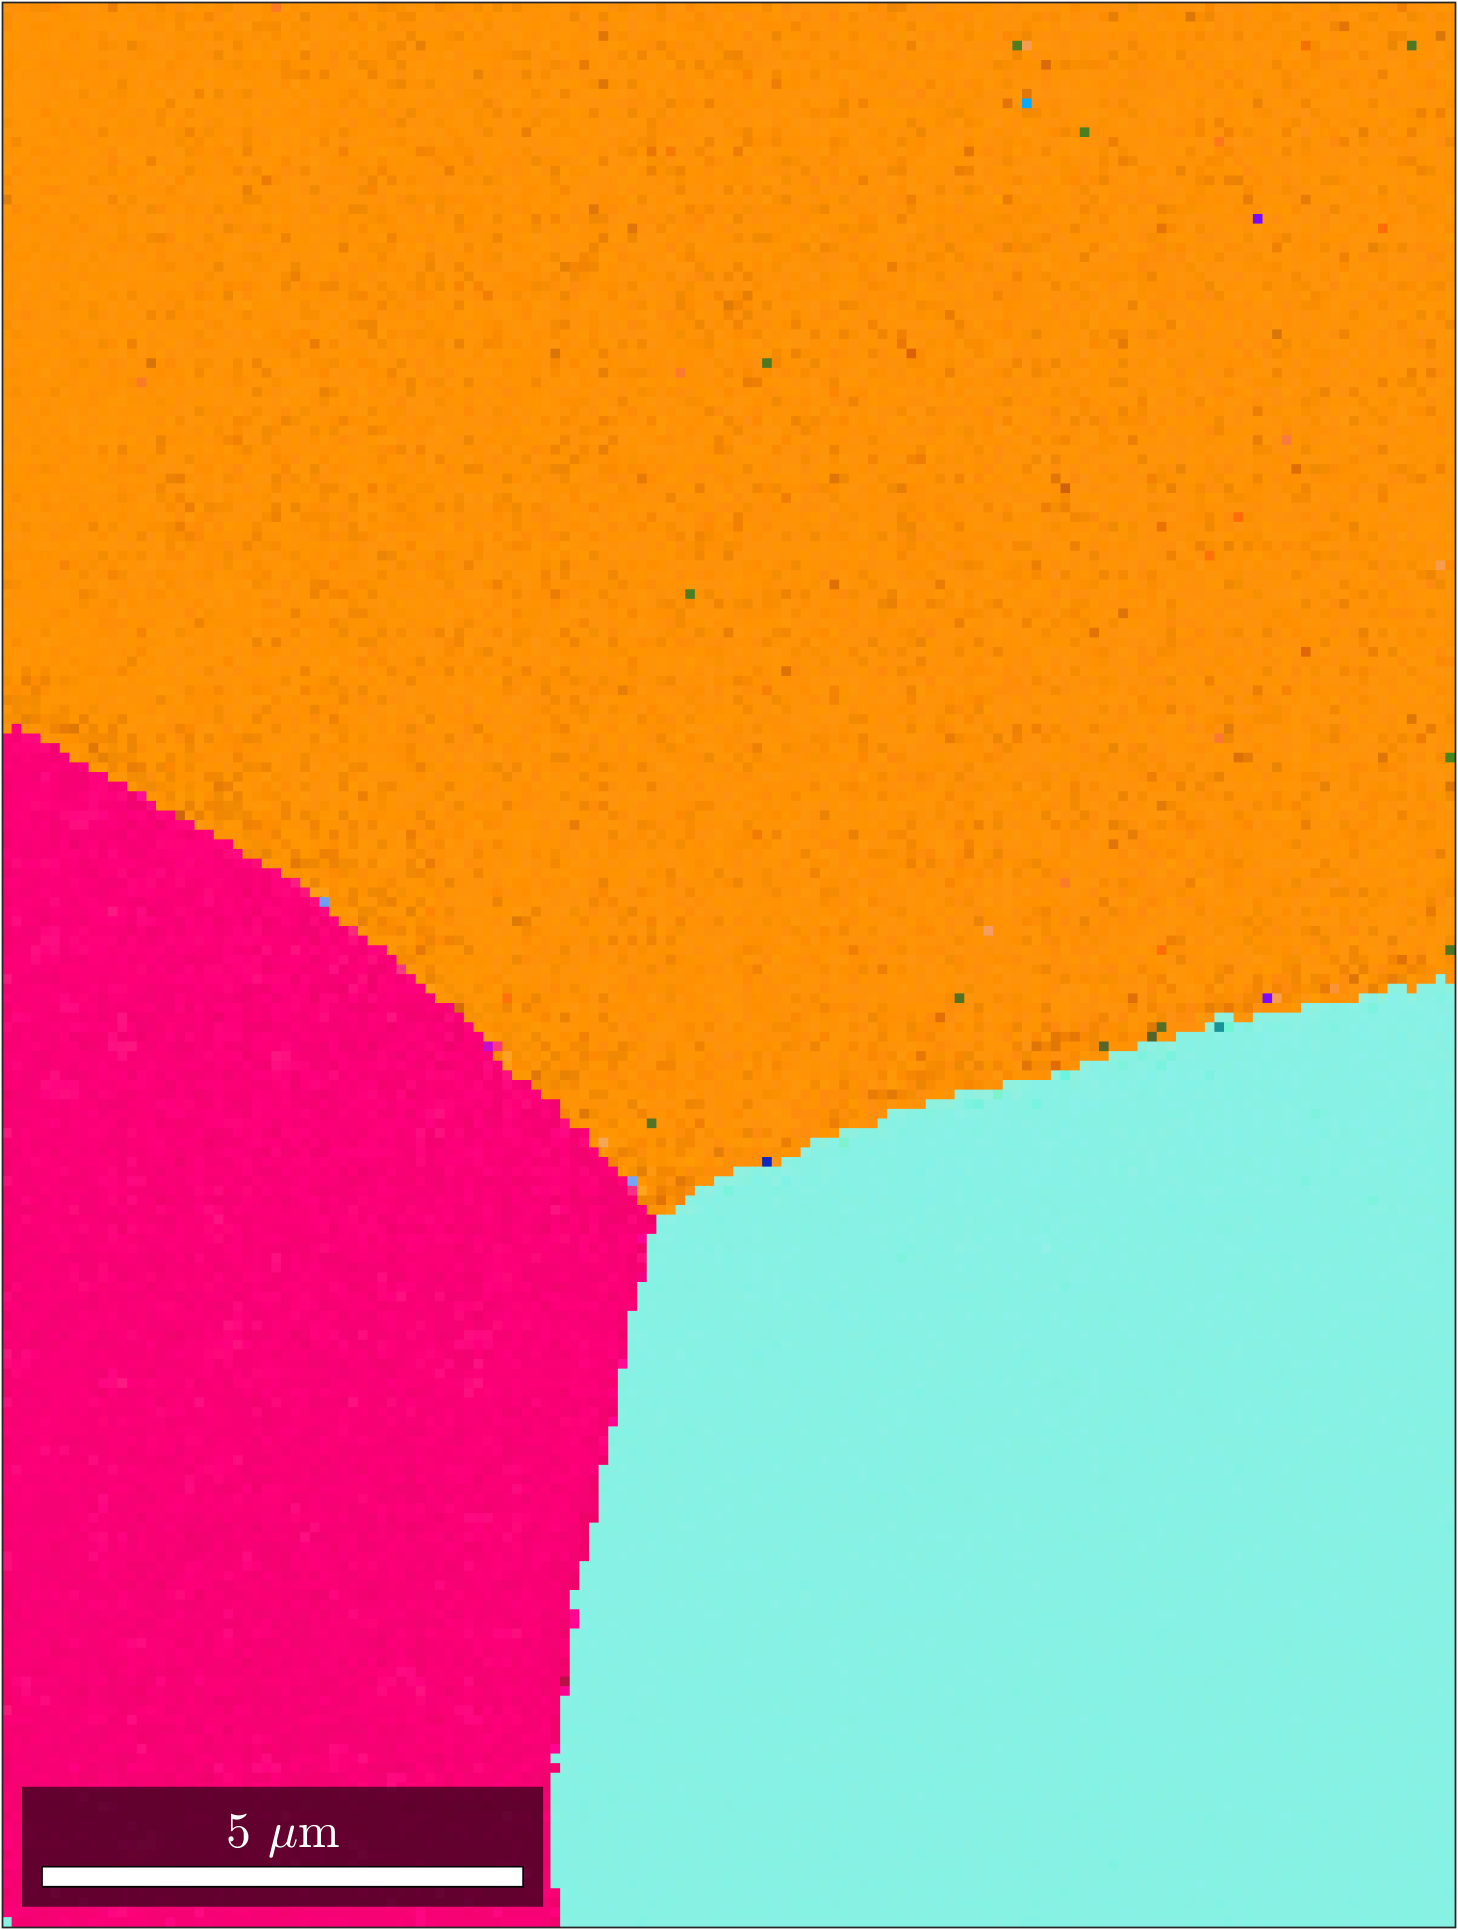
\includegraphics[width=\textwidth]{pic2/intro/ebsd1.png}
      \end{onlyenv}
      \begin{onlyenv}<2>
        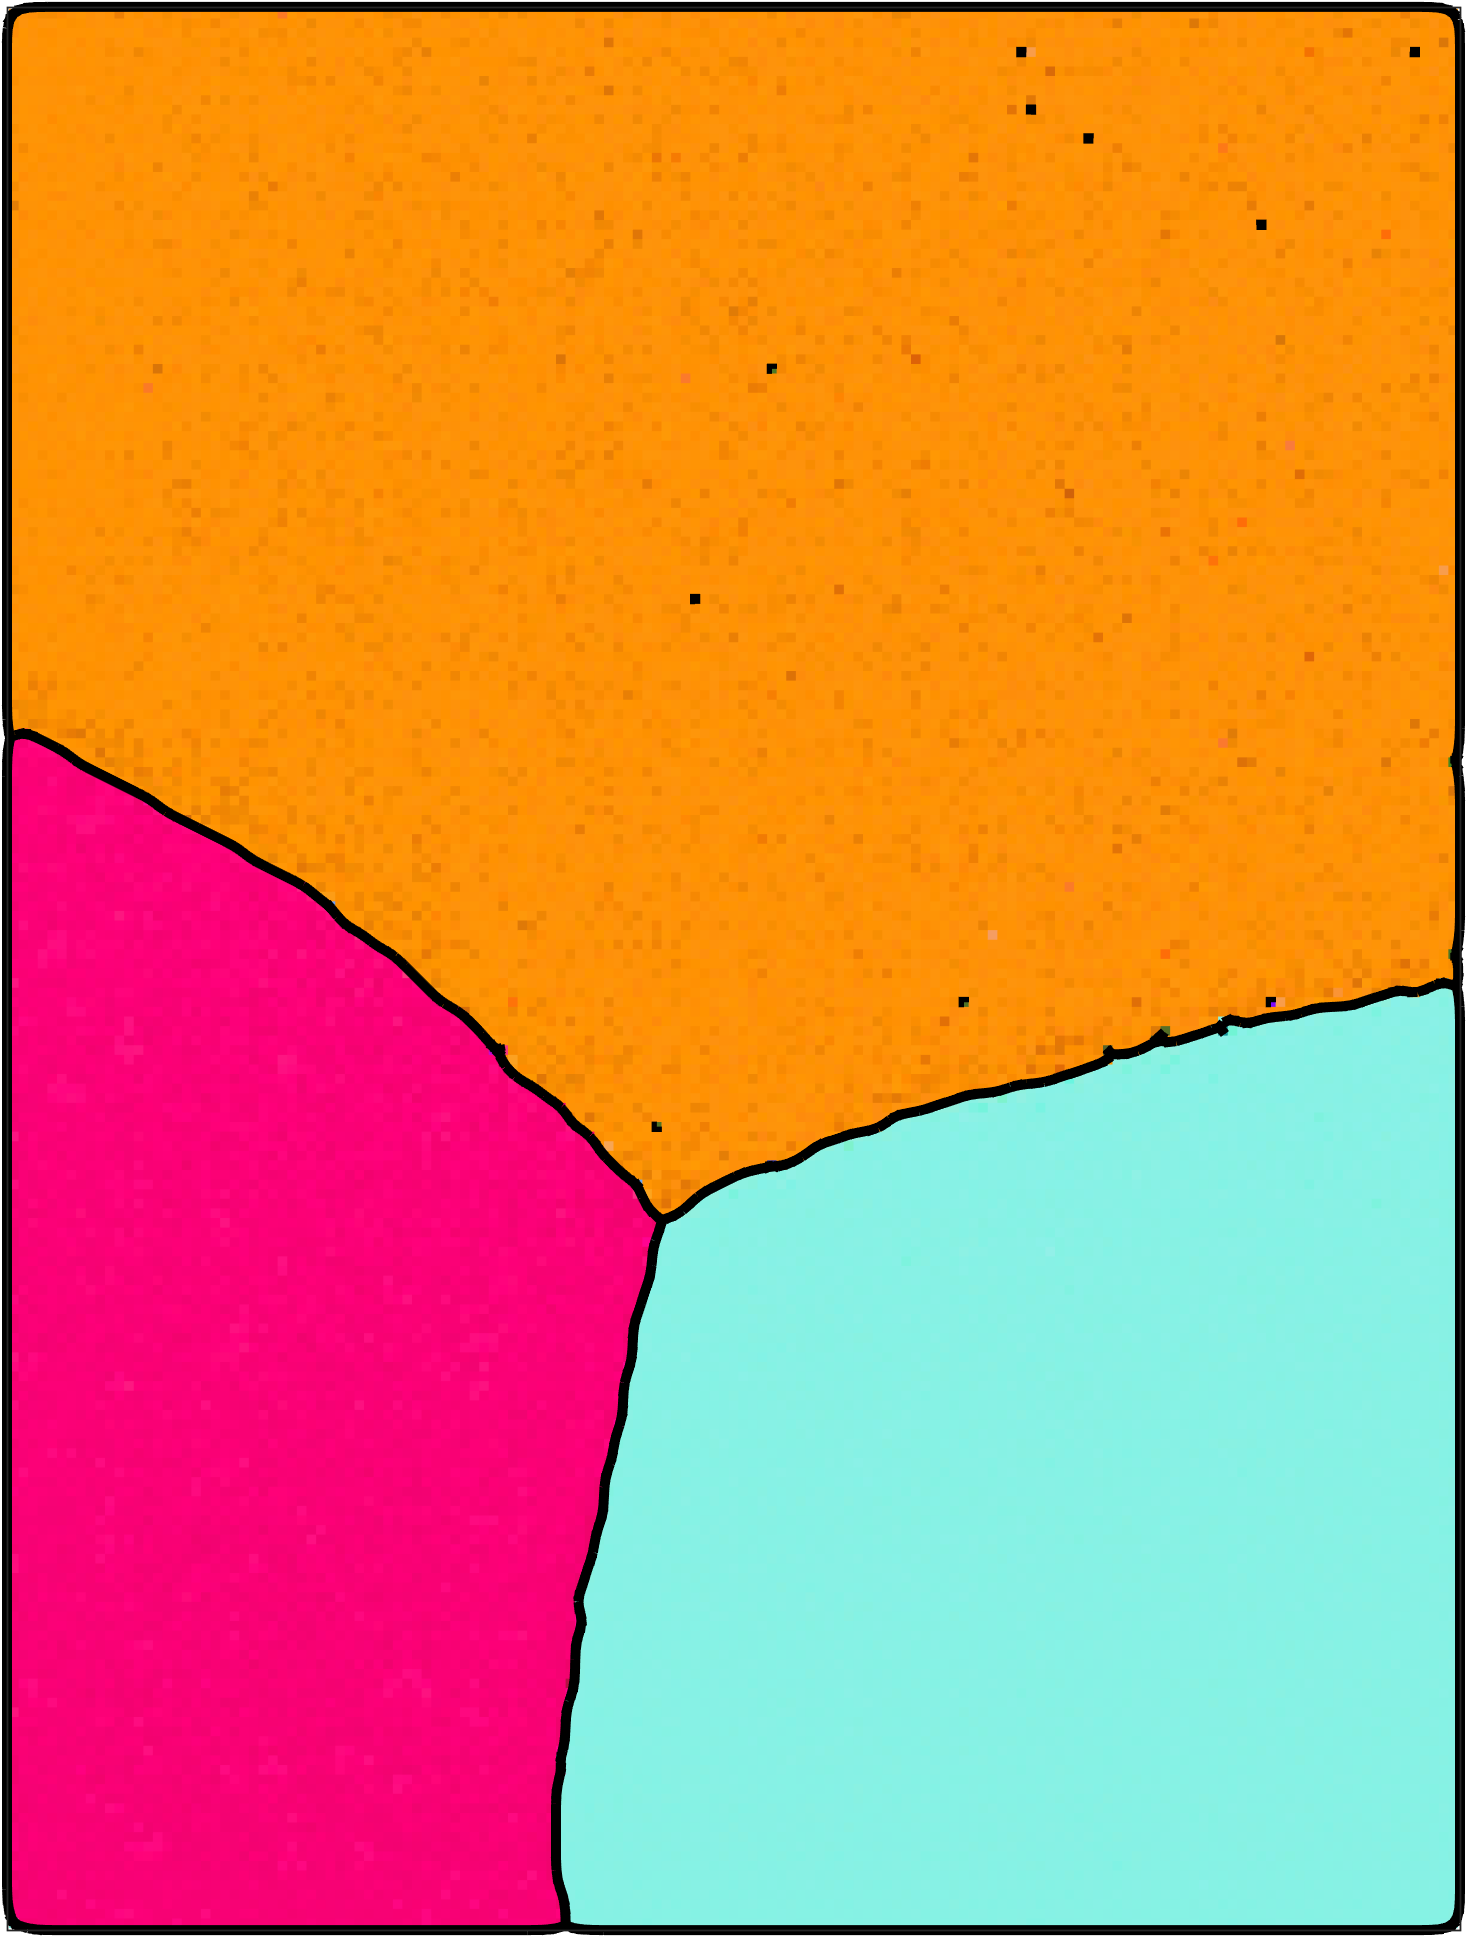
\includegraphics[width=\textwidth]{pic2/intro/ebsd1Grains.png}
      \end{onlyenv}
      \begin{onlyenv}<3>
        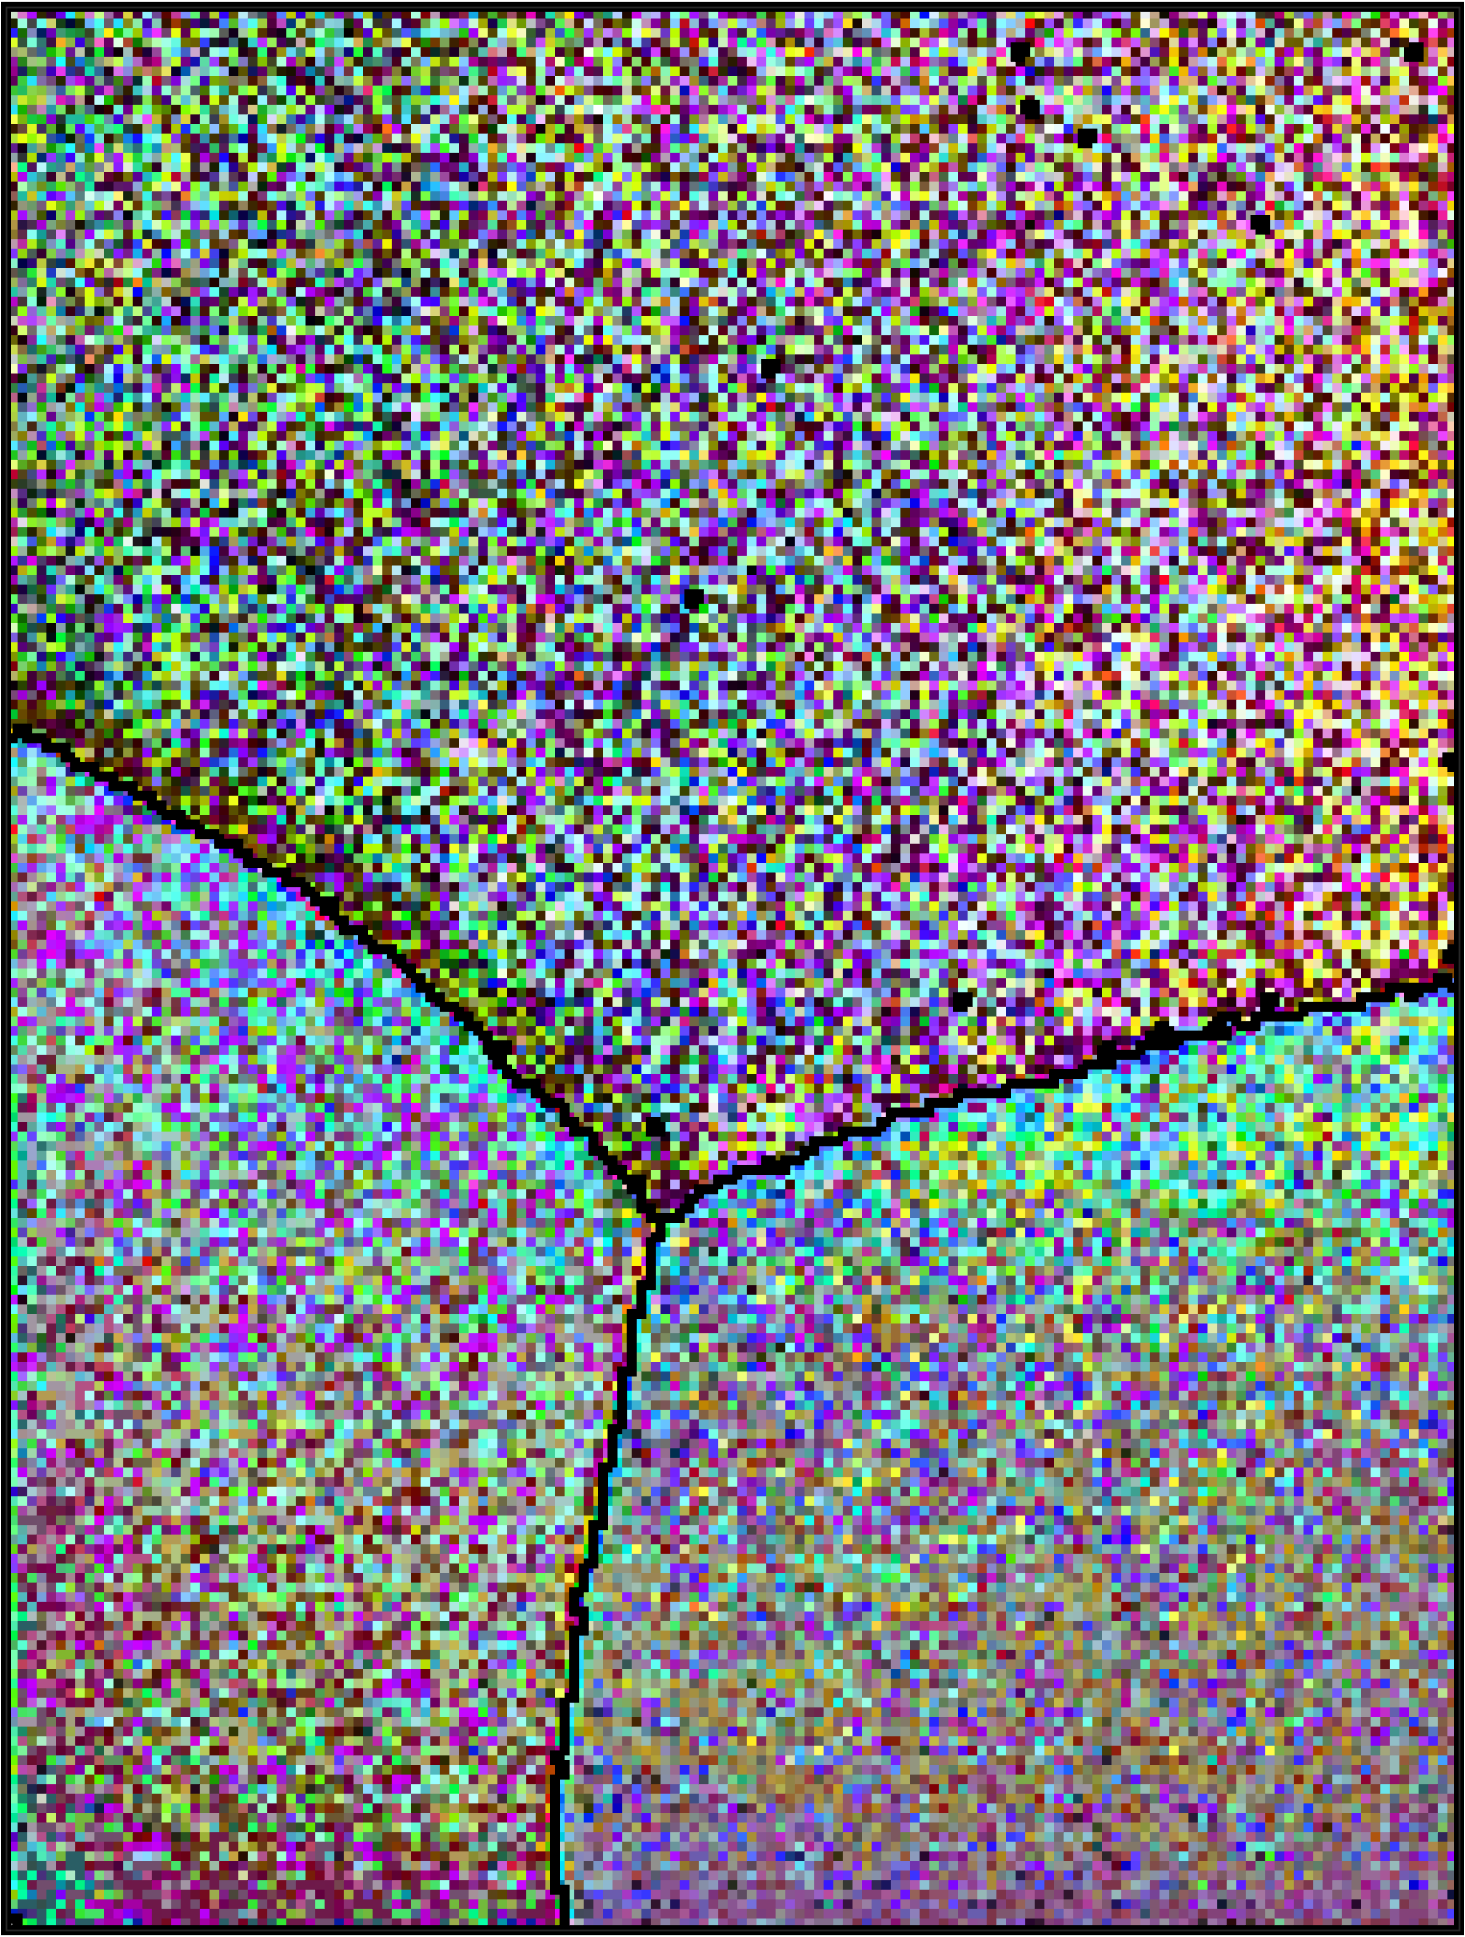
\includegraphics[width=\textwidth]{pic2/intro/ebsd1mis2mean.png}
      \end{onlyenv}
      \begin{onlyenv}<4>
        \vspace{-0.2cm}
        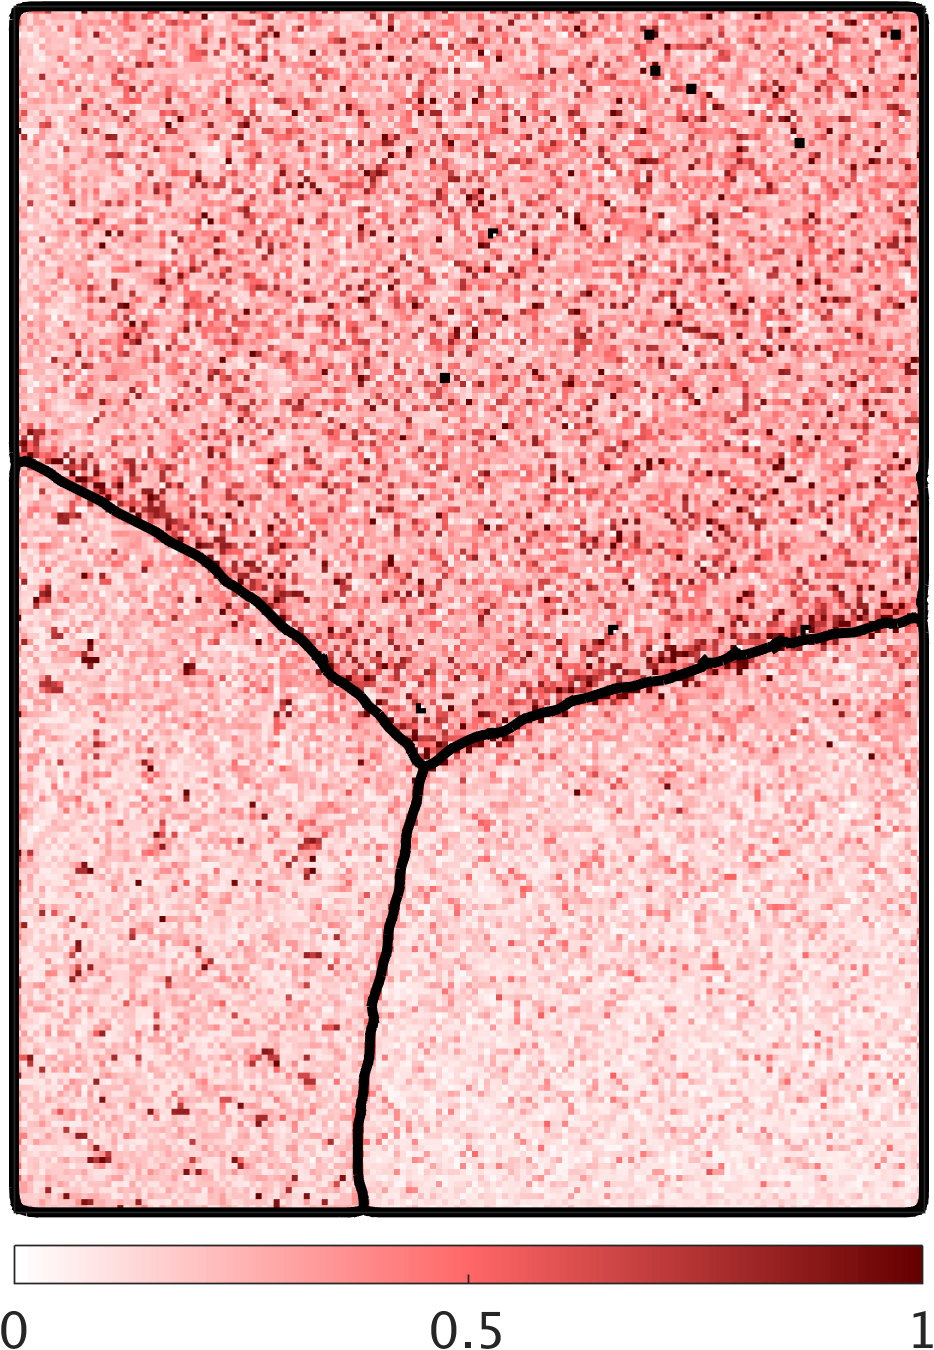
\includegraphics[width=0.87\textwidth]{pic2/intro/ebsd1KAM.png}
      \end{onlyenv}
      \begin{onlyenv}<5>
        \vspace{-0.2cm}
        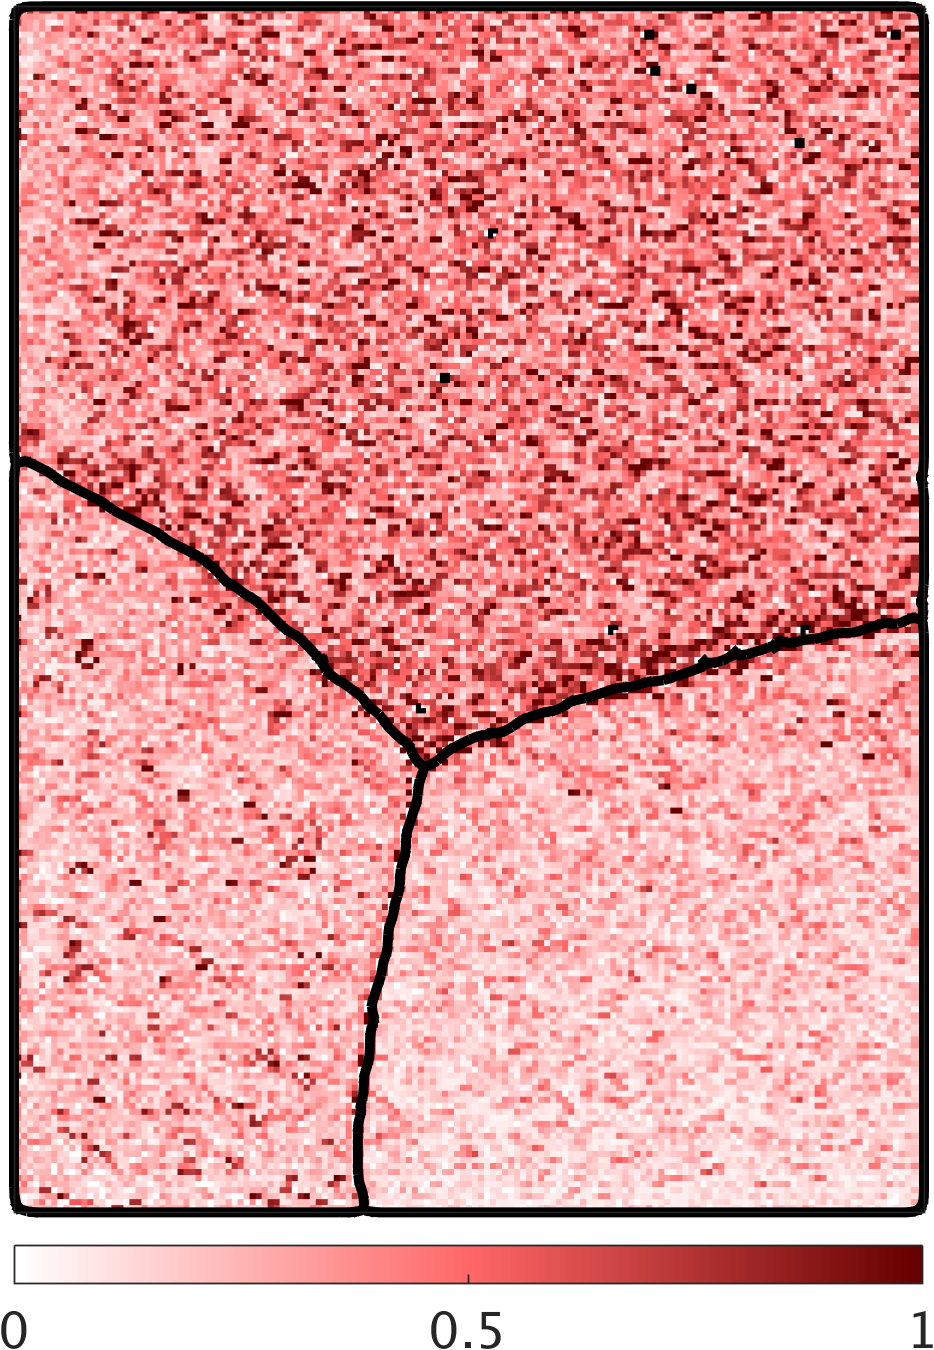
\includegraphics[width=0.87\textwidth]{pic2/intro/ebsd1gradientX.png}
      \end{onlyenv}
      \begin{onlyenv}<6>
        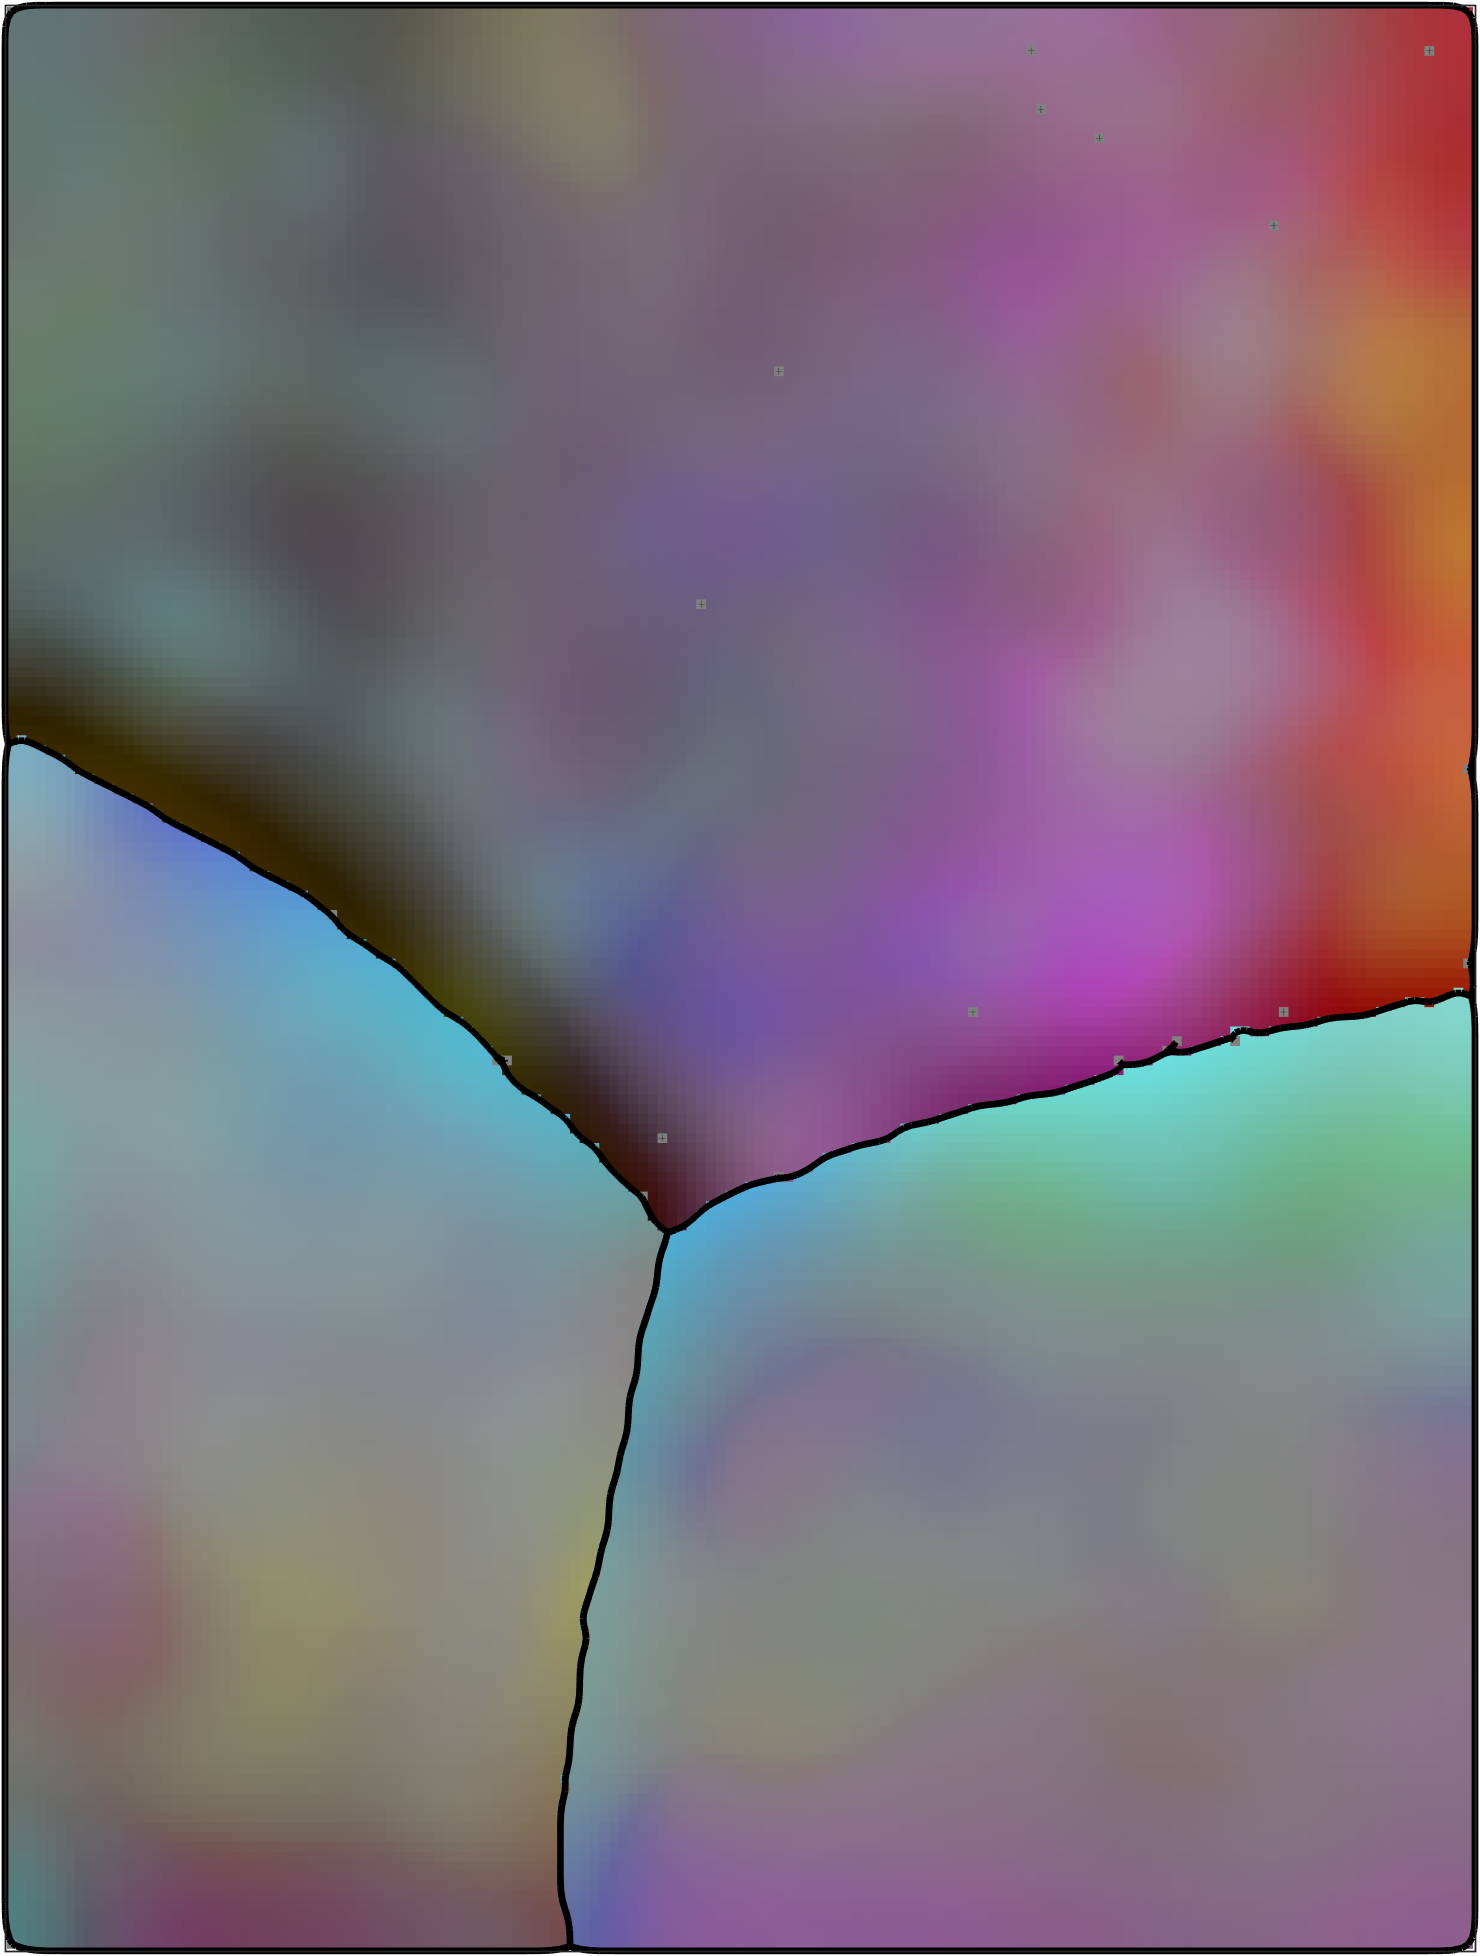
\includegraphics[width=\textwidth]{pic2/intro/ebsd1Spline.png}
      \end{onlyenv}
      \begin{onlyenv}<7>
        \vspace{-0.2cm}
        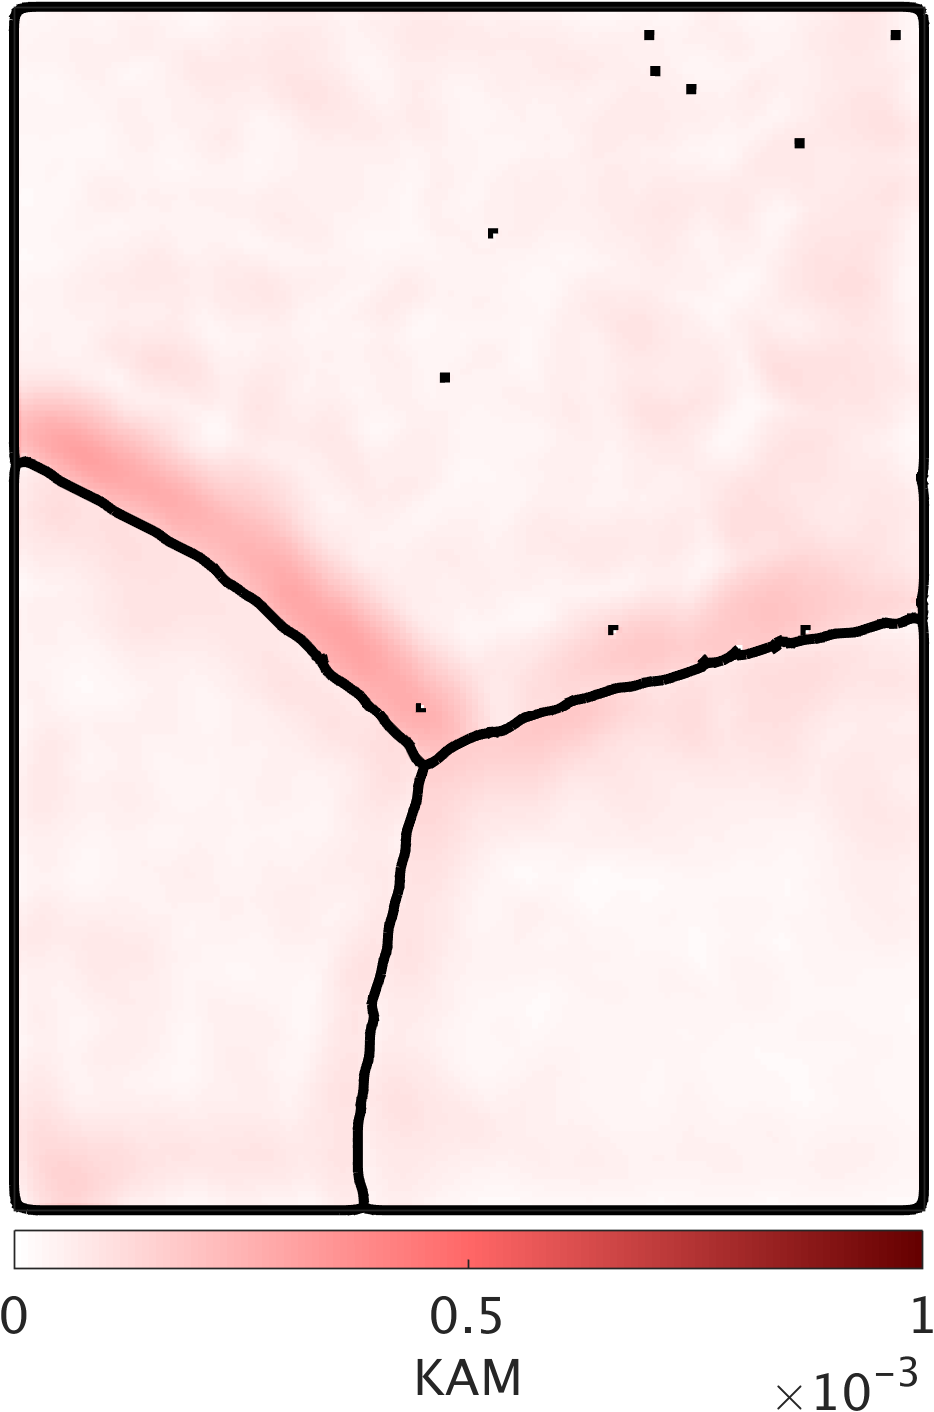
\includegraphics[width=0.87\textwidth]{pic2/intro/ebsd1SmoothedKAM.png}
      \end{onlyenv}
    \end{column}
  \end{columns}

\end{frame}


\begin{frame}
  \frametitle{An Academic Example}


  \begin{columns}
    \begin{column}{0.3\textwidth}

    \begin{tikzpicture}
      \begin{axis}[width=1.35\textwidth,height=4.5cm, ymin=-20,ymax=20,xmax=100,enlargelimits=false,
        cycle list name=exotic,legend pos=south west,hide x axis, hide y axis,
        legend style={cells={anchor=west}}]
        \addplot+[mark=none] table[x index=0,y index=1]{sim/raw.txt};
        \addplot graphics [ymin=-20,ymax=-1,xmin=0,xmax=100]{./sim/sim.png};
      \end{axis}
    \end{tikzpicture}
    \begin{block}{true data}
      \begin{itemize}
      \item $100 \times 25$ pixels
      \item $18^{\circ}$ grain boundary
      \end{itemize}
    \end{block}
    \end{column}
  \begin{column}{0.3\textwidth}
    \begin{tikzpicture}
      \begin{axis}[width=1.35\textwidth,height=4.5cm, ymin=-20,ymax=20,xmax=100,enlargelimits=false,
        cycle list name=exotic,legend pos=south west,hide x axis, hide y axis,
        legend style={cells={anchor=west}}]
        \addplot+[mark=none] table[x index=0,y index=2]{./sim/raw.txt};
        \addplot graphics [ymin=-20,ymax=-1,xmin=0,xmax=100]{./sim/poussin.png};
      \end{axis}
    \end{tikzpicture}
        \begin{block}{Gausian type noise}
      \begin{itemize}
      \item de la Vallee Poussin
      \item halfwidth $1^{\circ}$
      \end{itemize}
    \end{block}
  \end{column}
    \begin{column}{0.3\textwidth}
    \begin{tikzpicture}
      \begin{axis}[width=1.35\textwidth,height=4.5cm,ymin=-20,ymax=20,xmax=100,enlargelimits=false,
      %\begin{axis}[width=0.8\textwidth,height=3.4cm, ymin=-20,ymax=20,xmax=100,enlargelimits=false,
        cycle list name=exotic,legend pos=south west,hide x axis, hide y axis,
        legend style={cells={anchor=west}}]
        \addplot+[mark=none] table[x index=0,y index=3]{./sim/raw.txt};
        \addplot graphics [ymin=-20,ymax=-1,xmin=0,xmax=100]{./sim/saltPepper.png};
      \end{axis}
    \end{tikzpicture}
    \begin{block}{salt and pepper noise}
      \begin{itemize}
      \item $5\%$ missindexed pixels
      \item random orientation
      \end{itemize}
    \end{block}
    \end{column}

  \end{columns}

\end{frame}


\begin{frame}
  \frametitle{Sliding Window Techniques for EBSD Denoising}

  % sliding windows!!

  \begin{overlayarea}{\textwidth}{4.5cm}
    \begin{enumerate}
    \item<+-> \structure{the mean filter:} mean of
      neighbors

      \vspace{0.2cm}
      Gaussian noise \checked \hspace{0.2cm}
      grain boundaries \crossed \hspace{0.2cm}
      missindexed pixels \crossed \hspace{0.2cm}
      gradients \checked
      \vspace{0.2cm}

    \item<+-> \structure{the Kuwahara filter:} mean with
      smallest variance

      \vspace{0.2cm}
      Gaussian noise \crossed \hspace{0.2cm}
      grain boundaries \checked \hspace{0.2cm}
      missindexed pixels \crossed \hspace{0.2cm}
      gradients \crossed
      \vspace{0.2cm}

    \item<+-> \structure{the median filter:} neighboring
      orientation with minimum variance

      \vspace{0.2cm}
      Gaussian noise \crossed \hspace{0.2cm}
      grain boundaries \checked \hspace{0.2cm}
      missindexed pixels \checked \hspace{0.2cm}
      gradients \crossed
      \vspace{0.2cm}

    \end{enumerate}
  \end{overlayarea}

   \begin{center}
   \begin{onlyenv}<1>
      \begin{tikzpicture}
        \begin{axis}[width=0.4\textwidth,height=4.5cm,
          ymin=-20,ymax=20,xmax=100,enlargelimits=false, cycle list
          name=exotic,legend pos=south west,hide x axis, hide y axis, legend
          style={cells={anchor=west}}]
          \addplot+[mark=none] table[x index=0,y index=1]{./sim/mean.txt};
          \addplot graphics
          [ymin=-20,ymax=-1,xmin=0,xmax=100]{./sim/mean1.png};
        \end{axis}
      \end{tikzpicture}
      \begin{tikzpicture}
        \begin{axis}[width=0.4\textwidth,height=4.5cm,
          ymin=-20,ymax=20,xmax=100,enlargelimits=false, cycle list
          name=exotic,legend pos=south west,hide x axis, hide y axis, legend
          style={cells={anchor=west}}]
          \addplot+[mark=none] table[x index=0,y index=3]{./sim/mean.txt};
          \addplot graphics
          [ymin=-20,ymax=-1,xmin=0,xmax=100]{./sim/mean3.png};
        \end{axis}
      \end{tikzpicture}
      \begin{tikzpicture}
        \begin{axis}[width=0.4\textwidth,height=4.5cm,
          ymin=-20,ymax=20,xmax=100,enlargelimits=false, cycle list
          name=exotic,legend pos=south west,hide x axis, hide y axis, legend
          style={cells={anchor=west}}]
          \addplot+[mark=none] table[x index=0,y index=4]{./sim/mean.txt};
          \addplot graphics
          [ymin=-20,ymax=-1,xmin=0,xmax=100]{./sim/meanSP.png};
        \end{axis}
      \end{tikzpicture}
       \end{onlyenv}
        \begin{onlyenv}<2>
          \begin{tikzpicture}
      \begin{axis}[width=0.4\textwidth,height=4.5cm, ymin=-20,ymax=20,xmax=100,enlargelimits=false,
        cycle list name=exotic,legend pos=south west,hide x axis, hide y axis,
        legend style={cells={anchor=west}}]
        \addplot+[mark=none] table[x index=0,y index=1]{./sim/kuwaSec.txt};
        \addplot graphics [ymin=-20,ymax=-1,xmin=0,xmax=100]{./sim/kuwa1.png};
      \end{axis}
    \end{tikzpicture}
    \begin{tikzpicture}
      \begin{axis}[width=0.4\textwidth,height=4.5cm, ymin=-20,ymax=20,xmax=100,enlargelimits=false,
        cycle list name=exotic,legend pos=south west,hide x axis, hide y axis,
        legend style={cells={anchor=west}}]
        \addplot+[mark=none] table[x index=0,y index=3]{./sim/kuwaSec.txt};
        \addplot graphics [ymin=-20,ymax=-1,xmin=0,xmax=100]{./sim/kuwa3.png};
      \end{axis}
    \end{tikzpicture}
    \begin{tikzpicture}
      \begin{axis}[width=0.4\textwidth,height=4.5cm,
        ymin=-20,ymax=20,xmax=100,enlargelimits=false, cycle list
        name=exotic,legend pos=south west,hide x axis, hide y axis, legend
        style={cells={anchor=west}}]
        \addplot+[mark=none] table[x index=0,y index=4]{./sim/kuwaSec.txt};
        \addplot graphics [ymin=-20,ymax=-1,xmin=0,xmax=100]{./sim/kuwaSP.png};
      \end{axis}
    \end{tikzpicture}
  \end{onlyenv}
  % ----------------- median -------------------------
  \begin{onlyenv}<3>
    \begin{tikzpicture}
      \begin{axis}[width=0.4\textwidth,height=4.5cm, ymin=-20,ymax=20,xmax=100,enlargelimits=false,
        cycle list name=exotic,legend pos=south west,hide x axis, hide y axis,
        legend style={cells={anchor=west}}]
        \addplot+[mark=none] table[x index=0,y index=1]{./sim/medianSec.txt};
        \addplot graphics [ymin=-20,ymax=-1,xmin=0,xmax=100]{./sim/median1.png};
      \end{axis}
    \end{tikzpicture}
    \begin{tikzpicture}
      \begin{axis}[width=0.4\textwidth,height=4.5cm, ymin=-20,ymax=20,xmax=100,enlargelimits=false,
        cycle list name=exotic,legend pos=south west,hide x axis, hide y axis,
        legend style={cells={anchor=west}}]
        \addplot+[mark=none] table[x index=0,y index=3]{./sim/medianSec.txt};
        \addplot graphics [ymin=-20,ymax=-1,xmin=0,xmax=100]{./sim/median3.png};
      \end{axis}
    \end{tikzpicture}
    \begin{tikzpicture}
      \begin{axis}[width=0.4\textwidth,height=4.5cm,
        ymin=-20,ymax=20,xmax=100,enlargelimits=false, cycle list
        name=exotic,legend pos=south west,hide x axis, hide y axis, legend
        style={cells={anchor=west}}]
        \addplot+[mark=none] table[x index=0,y index=4]{./sim/medianSec.txt};
        \addplot graphics [ymin=-20,ymax=-1,xmin=0,xmax=100]{./sim/medianSP.png};
      \end{axis}
    \end{tikzpicture}
  \end{onlyenv}
   \end{center}


\end{frame}

\begin{frame}
  \frametitle{Global Denoising Techniques}


  \begin{block}{methods from mathematical image analysis}
    \begin{itemize}
    \item approximation by Fourier series, splines, wavelets, shearlets
    \item discrete variational methods
    \end{itemize}
  \end{block}

  \pause

  \begin{block}{variational methods}
    Minimize the functional
    \vspace{0.3cm}
    \begin{equation*}
      J(\vec{O})
      = \sum_{i,j} \omega(\vec{\tilde O}_{ij},\vec{O}_{ij})^{2}
      + \alpha \cdot \varphi(\vec{O})
    \end{equation*}
    \begin{minipage}{0.45\linewidth}
      \begin{itemize}
      \item \structure{ $i,j$} - pixel indices
      \item \structure{ $\vec{\tilde O}_{ij}$} - noisy orientation image
      \item \structure{ $\vec O_{ij}$} - denoised orientation image
    \end{itemize}
    \end{minipage}
    \begin{minipage}{0.45\linewidth}
      \begin{itemize}
      \item \structure{$\omega(\vec{\tilde O}_{ij},\vec{ O}_{ij})$} - misorientation angle
      \item \structure{$\varphi(\vec{O})$} - smoothness of
      $\vec{O}$
    \item \structure{$\alpha$} - regularization parameter
    \end{itemize}
    \end{minipage}

  \end{block}

\end{frame}


\begin{frame}
  \frametitle{Smoothing Splines}

  \begin{block}{minimization functional}
    \begin{equation*}
      J(\vec{O})
      = \sum_{i,j} \omega(\vec{\tilde O}_{ij},\vec{
          O}_{ij})^{2}
      + \alpha  (\triangle \vec{O}_{ij})^{2}
    \end{equation*}
  \end{block}


  \begin{multicols}{3}
    \begin{itemize}
    \item[\checked] Gaussian Noise
    \item[\checked] gradients
    \item[\crossed] grain boundaries
    \item[\checked] fast
    \item[\checked] missindexed pixels
    \item[\checked] $\alpha$ determination
    \end{itemize}
  \end{multicols}

  \bigskip

  % \begin{columns}
  %   \begin{column}{0.44\textwidth}
  %     \begin{itemize}
  %     \item[\checked] Gaussian noise
  %     \item[\crossed] grain boundaries
  %     \item[\checked] missindexed pixels
  %   \end{itemize}
  % \end{column}
  % \begin{column}{0.44\textwidth}
  %   \begin{itemize}
  %   \item[\checked] gradients
  %   \item[\checked] fast
  %   \item[\checked] automatic $\alpha$ estimation
  %   \end{itemize}
  %   \end{column}
  % \end{columns}


  \begin{center}
    \begin{tikzpicture}
      \begin{axis}[width=0.43\textwidth,height=4.9cm,
        ymin=-20,ymax=20,xmax=100,enlargelimits=false, cycle list
        name=exotic,legend pos=south west,hide x axis, hide y axis, legend
        style={cells={anchor=west}}]
        \addplot+[mark=none] table[x index=0,y index=2]{./sim/spline.txt};
        \addplot graphics
        [ymin=-20,ymax=-1,xmin=0,xmax=100]{./sim/spline2.png};
      \end{axis}
    \end{tikzpicture}
    \begin{tikzpicture}
      \begin{axis}[width=0.43\textwidth,height=4.9cm,
        ymin=-20,ymax=20,xmax=100,enlargelimits=false, cycle list
        name=exotic,legend pos=south west,hide x axis, hide y axis, legend
        style={cells={anchor=west}}]
        \addplot+[mark=none] table[x index=0,y index=3]{./sim/spline.txt};
        \addplot graphics
        [ymin=-20,ymax=-1,xmin=0,xmax=100]{./sim/spline3.png};
      \end{axis}
    \end{tikzpicture}
    \begin{tikzpicture}
      \begin{axis}[width=0.43\textwidth,height=4.9cm,
        ymin=-20,ymax=20,xmax=100,enlargelimits=false, cycle list
        name=exotic,legend pos=south west,hide x axis, hide y axis, legend
        style={cells={anchor=west}}]
        \addplot+[mark=none] table[x index=0,y index=4]{./sim/spline.txt};
        \addplot graphics
        [ymin=-20,ymax=-1,xmin=0,xmax=100]{./sim/splineSP.png};
      \end{axis}
    \end{tikzpicture}
  \end{center}


\end{frame}

\begin{frame}
  \frametitle{Total Variation}

\begin{block}{minimization functional}
    \begin{equation*}
      J(\vec{O})
      = \sum_{i,j} \omega(\vec{\tilde O}_{ij},\vec{
          O})^{\textcolor{darkred}{\mathbf{1}}}
      + \alpha \lVert\nabla \vec{O}_{ij}\rVert_{2}^{\textcolor{darkred}{\mathbf{1}}}
    \end{equation*}
  \end{block}


  \begin{multicols}{3}
    \begin{itemize}
    \item[\checked] Gaussian Noise
    \item[\ok] gradients
    \item[\checked] grain boundaries
    \item[\checked] currently fastest
    \item[\checked] missindexed pixels
    \item[\crossed] $\alpha$ required
    \end{itemize}
  \end{multicols}

\bigskip

%   \begin{columns}
%     \begin{column}{0.45\textwidth}
%       \begin{itemize}
%       \item[\checked] Gaussian Noise
%       \item[\checked] grain boundaries
%       \item[\crossed] missindexed pixels
%       \end{itemize}
%     \end{column}
%     \begin{column}{0.45\textwidth}
%       \begin{itemize}
%       \item[\ok] gradients
%       \item[\ok] not so fast
%       \item[\crossed] no automatic $\alpha$ estimation
% %      \item cartoon like images \ok
%     \end{itemize}
%     \end{column}
%   \end{columns}

  \begin{center}
    \begin{tikzpicture}
      \begin{axis}[width=0.43\textwidth,height=4.9cm,
        ymin=-20,ymax=20,xmax=100,enlargelimits=false, cycle list
        name=exotic,legend pos=south west,hide x axis, hide y axis, legend
        style={cells={anchor=west}}]
        \addplot+[mark=none] table[x index=0,y index=1]{./sim/halfquad.txt};
        \addplot graphics
        [ymin=-20,ymax=-1,xmin=0,xmax=100]{./sim/halfquad1.png};
      \end{axis}
    \end{tikzpicture}
    \begin{tikzpicture}
      \begin{axis}[width=0.43\textwidth,height=4.9cm,
        ymin=-20,ymax=20,xmax=100,enlargelimits=false, cycle list
        name=exotic,legend pos=south west,hide x axis, hide y axis, legend
        style={cells={anchor=west}}]
        \addplot+[mark=none] table[x index=0,y index=3]{./sim/halfquad.txt};
        \addplot graphics
        [ymin=-20,ymax=-1,xmin=0,xmax=100]{./sim/halfquad3.png};
      \end{axis}
    \end{tikzpicture}
    \begin{tikzpicture}
      \begin{axis}[width=0.43\textwidth,height=4.9cm,
        ymin=-20,ymax=20,xmax=100,enlargelimits=false, cycle list
        name=exotic,legend pos=south west,hide x axis, hide y axis, legend
        style={cells={anchor=west}}]
        \addplot+[mark=none] table[x index=0,y index=4]{./sim/halfquad.txt};
        \addplot graphics
        [ymin=-20,ymax=-1,xmin=0,xmax=100]{./sim/halfquadSP.png};
      \end{axis}
    \end{tikzpicture}
  \end{center}

\end{frame}

% \begin{frame}
%   \frametitle{Infimal Convolution}

% \begin{block}{minimization functional}
%     \begin{equation*}
%       J(\vec{U},\vec{V})
%       = \sum_{i,j} \omega(\vec{\tilde O}_{ij},\vec{U}_{ij} \vec{V}_{ij})^{2}
%       + \alpha \lVert\nabla \vec{U}_{ij}\rVert_{2}
%       + \beta \lvert \triangle \vec V_{ij} \rvert
%     \end{equation*}
%   \end{block}

%   Idea: split image $\vec O$ into a picewise constant image $\vec U$ and a
%   smooth image $\vec V$

%       \begin{multicols}{3}
%         \begin{itemize}
%         \item[\checked] Gaussian noise
%         \item[\checked] gradients
%          \item[\checked] grain boundaries
%          \item[\crossed] very slow
%          \item[\crossed] missindexed pixels
%          \item[\crossed] $\alpha$, $\beta$ required
%         \end{itemize}
%       \end{multicols}

%   \begin{center}
%     \begin{tikzpicture}
%       \begin{axis}[width=0.43\textwidth,height=4.9cm,
%         ymin=-20,ymax=20,xmax=100,enlargelimits=false, cycle list
%         name=exotic,legend pos=south west,hide x axis, hide y axis, legend
%         style={cells={anchor=west}}]
%         \addplot+[mark=none] table[x index=0,y index=1]{./sim/invconf.txt};
%         \addplot graphics
%         [ymin=-20,ymax=-1,xmin=0,xmax=100]{./sim/infconv1.png};
%       \end{axis}
%     \end{tikzpicture}
%     \begin{tikzpicture}
%       \begin{axis}[width=0.43\textwidth,height=4.9cm,
%         ymin=-20,ymax=20,xmax=100,enlargelimits=false, cycle list
%         name=exotic,legend pos=south west,hide x axis, hide y axis, legend
%         style={cells={anchor=west}}]
%         \addplot+[mark=none] table[x index=0,y index=3]{./sim/invconf.txt};
%         \addplot graphics
%         [ymin=-20,ymax=-1,xmin=0,xmax=100]{./sim/infconv3.png};
%       \end{axis}
%     \end{tikzpicture}
%     \begin{tikzpicture}
%       \begin{axis}[width=0.43\textwidth,height=4.9cm,
%         ymin=-20,ymax=20,xmax=100,enlargelimits=false, cycle list
%         name=exotic,legend pos=south west,hide x axis, hide y axis, legend
%         style={cells={anchor=west}}]
%         \addplot+[mark=none] table[x index=0,y index=4]{./sim/invconf.txt};
%         \addplot graphics
%         [ymin=-20,ymax=-1,xmin=0,xmax=100]{./sim/invconfSP.png};
%       \end{axis}
%     \end{tikzpicture}
%   \end{center}

% \end{frame}



\begin{frame}
  \frametitle{Morphological Filter}


  \begin{overlayarea}{\textwidth}{7.5cm}
    \begin{onlyenv}<1-2>
      \begin{center}
        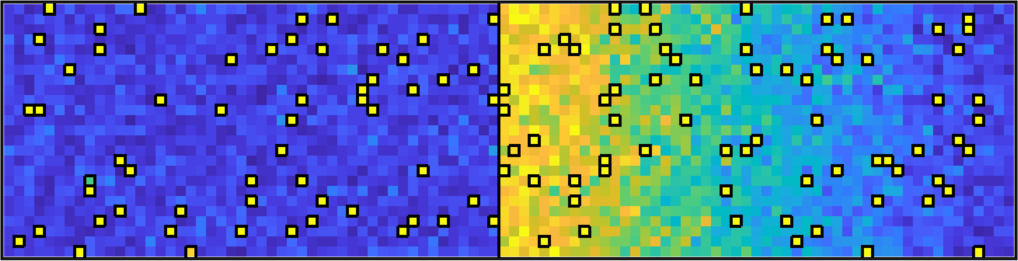
\includegraphics[width=0.45\textwidth]{./sim/grains.png}
        \quad
        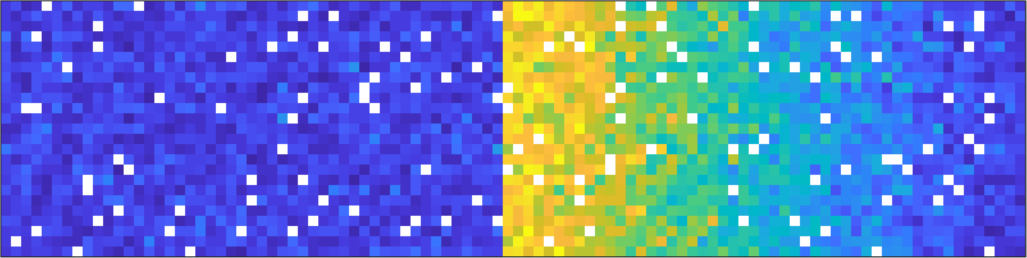
\includegraphics[width=0.45\textwidth]{./sim/grainsRemoved.png}
      \end{center}
    \end{onlyenv}

    \vspace{-0.6cm}
    \pause

    \begin{onlyenv}<2>
      \begin{center}
        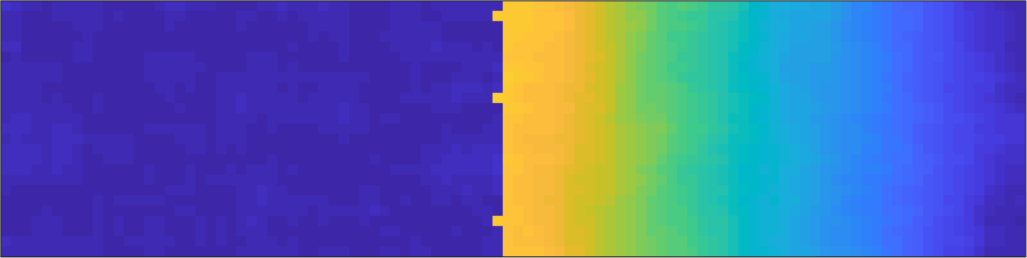
\includegraphics[width=0.45\textwidth]{./sim/meanGrain.png}
        \quad
        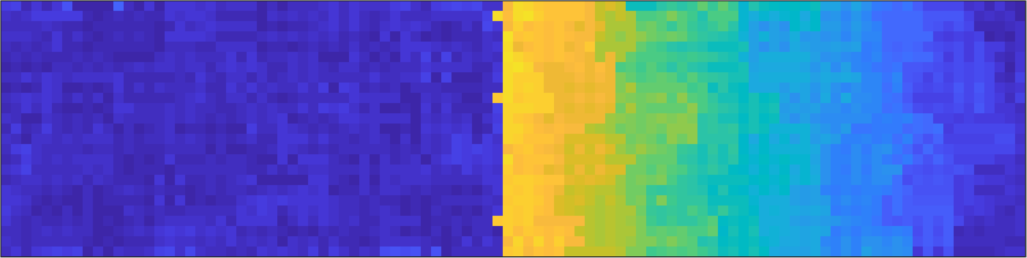
\includegraphics[width=0.45\textwidth]{./sim/kuwaharaGrain.png}

        \medskip

    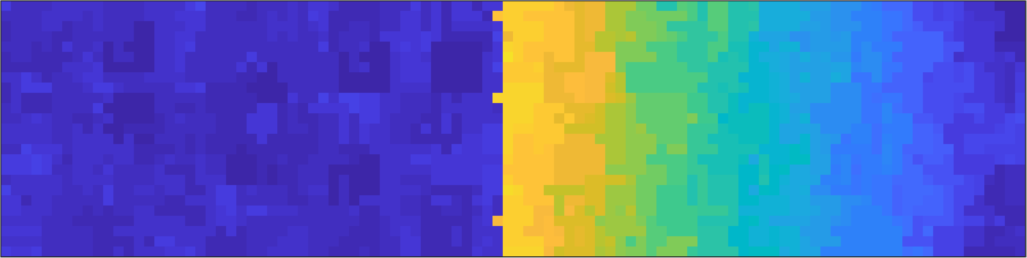
\includegraphics[width=0.45\textwidth]{./sim/medianGrain.png}
    \quad
    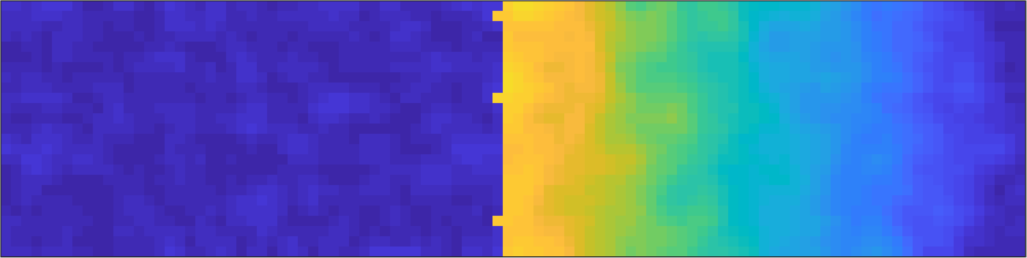
\includegraphics[width=0.45\textwidth]{./sim/splineGrain.png}

    \medskip

    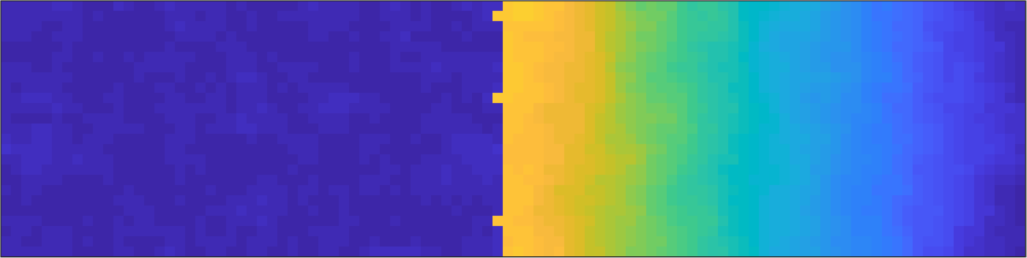
\includegraphics[width=0.45\textwidth]{./sim/halfquadGrain.png}
    \quad
    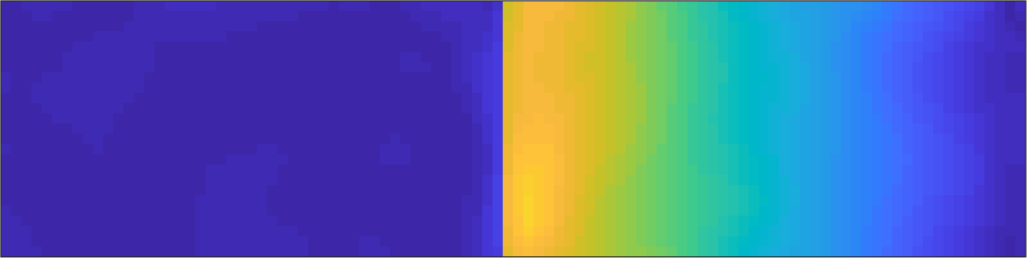
\includegraphics[width=0.45\textwidth]{./sim/infconvGrain.png}
  \end{center}
\end{onlyenv}
\end{overlayarea}
\end{frame}

% \begin{frame}
% \frametitle{A Real Grain}

%   \begin{onlyenv}<1>
%     \includegraphics[width=\textwidth]{pic/ggRaw.png}

%     \begin{center}
%       The raw data
%     \end{center}
%   \end{onlyenv}
%   \begin{onlyenv}<2>
%     \includegraphics[width=\textwidth]{pic/ggMean.png}

%     \begin{center}
%       The mean filter
%     \end{center}
%   \end{onlyenv}

%   \begin{onlyenv}<3>
%     \includegraphics[width=\textwidth]{pic/ggMedian.png}

%     \begin{center}
%       The median filter
%     \end{center}
%   \end{onlyenv}
%     \begin{onlyenv}<4>
%       \includegraphics[width=\textwidth]{pic2/ggSpline.png}

%       \begin{center}
%         The spline filter
%       \end{center}
%   \end{onlyenv}
%     \begin{onlyenv}<5>
%       \includegraphics[width=\textwidth]{pic2/gghalfQuad.png}

%           \begin{center}
%       The total variation filter
%     \end{center}
%   \end{onlyenv}
%     \begin{onlyenv}<6>
%       \includegraphics[width=\textwidth]{pic2/gginfimal.png}

%       \begin{center}
%       The infimal convolution filter
%     \end{center}
%   \end{onlyenv}


% \end{frame}

\begin{frame}
  \frametitle{A deformed grain}

  \begin{overlayarea}{\textwidth}{\textheight}

    \includegraphics<1->[height=0.45\textheight]{pic2/singleGrain/grainRaw.png}
    \;\pause
    \includegraphics<2->[height=0.45\textheight]{pic2/singleGrain/grainHalfQuad.png}
    \;\pause
    \includegraphics<3->[height=0.45\textheight]{pic2/singleGrain/grainMis2Mean.png}

    \pause

    \includegraphics<4->[height=0.45\textheight]{pic2/singleGrain/grainRaw10.png}
    \;\pause
    \includegraphics<5->[height=0.45\textheight]{pic2/singleGrain/grainSmooth10.png}
    \;\pause
    \includegraphics<6->[height=0.45\textheight]{pic2/singleGrain/grainSmooth10Error.png}

  \end{overlayarea}

\end{frame}



\begin{frame}
  \frametitle{Not Indexed Data}
  \begin{overlayarea}{\textwidth}{\textheight}


    \includegraphics<1->[height=0.45\textheight]{pic2/singleGrain/grainRaw50.png}
    \;\pause
    \includegraphics<2->[height=0.45\textheight]{pic2/singleGrain/grainSmooth50.png}
    \;\pause
    \includegraphics<3->[height=0.45\textheight]{pic2/singleGrain/grainSmooth50Error.png}

    \pause

    \includegraphics<4->[height=0.45\textheight]{pic2/singleGrain/grainRaw90.png}
    \;\pause
    \includegraphics<5->[height=0.45\textheight]{pic2/singleGrain/grainSmooth90.png}
    \;\pause
    \includegraphics<6->[height=0.45\textheight]{pic2/singleGrain/grainSmooth90Error.png}


  \end{overlayarea}

\end{frame}

\begin{frame}[fragile]
  %\frametitle{A Multigrain Example}


  \begin{overlayarea}{\textwidth}{0.9\textheight}
    \begin{center}
      \includegraphics<1>[width=0.8\textwidth]{pic2/ebsdGrainRaw.png}%
      \includegraphics<2>[width=0.8\textwidth]{pic2/ebsdGrain1.png}%
      \includegraphics<3>[width=0.8\textwidth]{pic2/ebsdGrain2.png}%
      \includegraphics<4>[width=0.8\textwidth]{pic2/ebsdGrain5.png}%
      \includegraphics<5>[width=0.8\textwidth]{pic2/FoAxisAngle.png}%
      \includegraphics<6>[width=0.8\textwidth]{pic2/FoMean.png}%
      \includegraphics<7>[width=0.8\textwidth]{pic2/FoMedian.png}%
      \includegraphics<8>[width=0.8\textwidth]{pic2/FoKuwahara.png}%
      \includegraphics<9>[width=0.8\textwidth]{pic2/FoSpline.png}%
      \includegraphics<10>[width=0.8\textwidth]{pic2/FoHalfQuad.png}%
      \includegraphics<11>[width=0.8\textwidth]{pic2/FoAxisAngle.png}%
      % \includegraphics<10>[width=\textwidth]{pic2/FoGrain6.png}
      % \includegraphics<6>[width=\textwidth]{pic2/emptyGrainIndex.png}
      % \includegraphics<7>[width=\textwidth]{pic2/ebsdGrain3.png}
    \end{center}
    \begin{center}
      \vspace{-0.3cm}
      \begin{onlyenv}<1> raw geological Forsterite data - white pixels are not
        indexed
      \end{onlyenv}
      \begin{onlyenv}<2> naiv grain reconstruction algorithm
      \end{onlyenv}
      \begin{onlyenv}<3> \structure{\small{Bachmann, Hielscher, Schaeben:
            Grain detection from 2d and 3d {EBSD} data, Ultramicroscopy,
            2011}}
      \end{onlyenv}
      \begin{onlyenv}<4> \centering{denoising and inpainting using smoothing
          splines}
      \end{onlyenv}
      \begin{onlyenv}<5,11> raw data, misorientation to grain mean orientation
      \end{onlyenv}
      \begin{onlyenv}<6> denoising and inpainting using the \structure{mean
          filter} with $5 \times 5$ window
      \end{onlyenv}
      \begin{onlyenv}<7> denoising and inpainting using the \structure{median
          filter} with $7 \times 7$ window
      \end{onlyenv}
      \begin{onlyenv}<8> denoising and inpainting using the
        \structure{Kuwahara filter} with $7 \times 7$ window
      \end{onlyenv}
      \begin{onlyenv}<9> denoising and inpainting using \structure{smoothing
          splines}
      \end{onlyenv}
      \begin{onlyenv}<10> denoising and inpainting using \structure{total
          variation}
      \end{onlyenv}
    \end{center}
    \end{overlayarea}
\end{frame}


\section{Orientation Gradients}

\subsection{Kernel Average Misorientation}

\begin{frame}
\frametitle{The Kernel Averaged Misorientation of Noisy Data}

\begin{minipage}{0.485\linewidth}

  noise free data:\\
  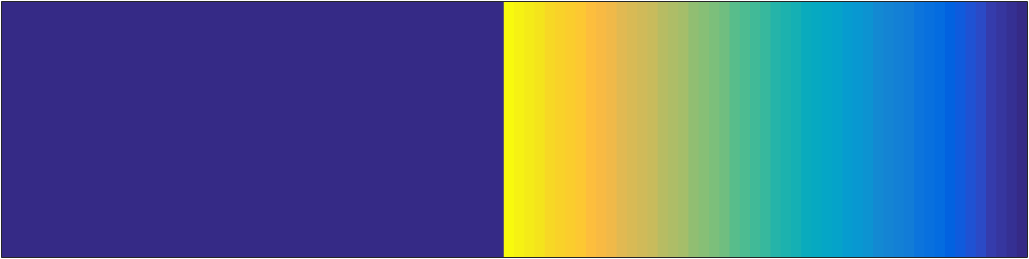
\includegraphics[height=1.6cm]{pic2/sim.png}

  \medskip

  KAM:\\
    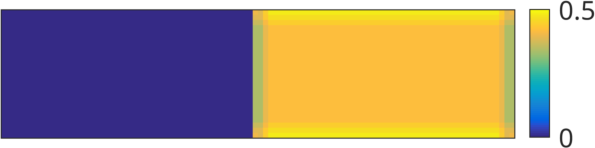
\includegraphics[height=1.83cm]{pic2/kamSimNoiseFree}
  \end{minipage}\hspace{0.3cm}%
  \begin{onlyenv}<2>%
    \begin{minipage}{0.485\linewidth}

      data with 1 degree noise:\\
      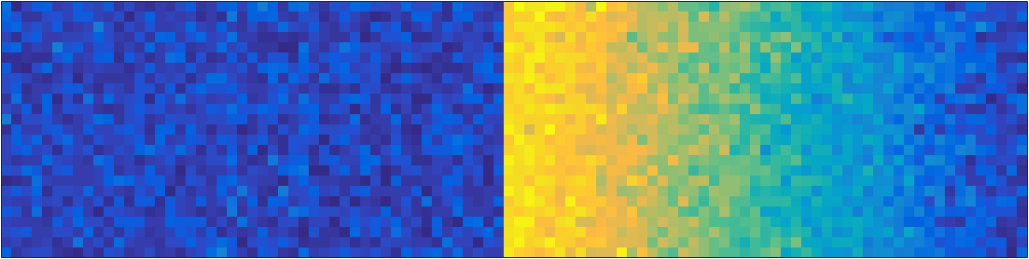
\includegraphics[height=1.6cm]{pic2/simNoise.png}

      \medskip

      KAM:\\
      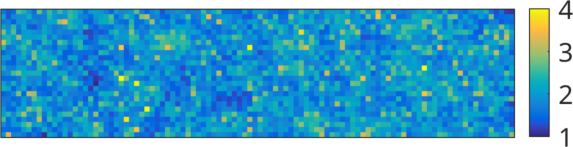
\includegraphics[height=1.84cm]{pic2/kamSimNoise}
    \end{minipage}
  \end{onlyenv}


\end{frame}



\begin{frame}
  \frametitle{The KAM of Noisy Data}
    \centering
    \begin{tikzpicture}
    \begin{axis}[width=\textwidth,height=7cm, ymin=-0.1,ymax=2.5,xmax=100,enlargelimits=false,
      cycle list name=exotic,
      legend columns = 5,
      legend style={at={(0.5,-0.2)},anchor=north}]
      \addplot+[mark=none, very thick] table[x index=0,y index=1]{pic2/kamSim.txt};
      \addplot+[mark=none, thick] table[x index=0,y index=2]{pic2/kamSim.txt};
      \addplot+[mark=none, thick] table[x index=0,y index=3]{pic2/kamSim.txt};
      \addplot+[mark=none, thick] table[x index=0,y index=4]{pic2/kamSim.txt};
      \addplot+[mark=none, thick] table[x index=0,y index=5]{pic2/kamSim.txt};
      \legend{no noise, $\delta = 0.25^{\circ}$, $\delta = 0.5^{\circ}$, $\delta = 0.75^{\circ}$, $\delta = 1^{\circ}$}
    \end{axis}
  \end{tikzpicture}
\end{frame}

  \begin{frame}
  \frametitle{The KAM of Denoised Data}
      \begin{tikzpicture}
    \begin{axis}[width=\textwidth,height=7cm, ymin=0,ymax=2.5,xmax=100,enlargelimits=false,
      cycle list name=exotic,legend pos=south west,
      legend columns = 5,
      legend style={at={(0.5,-0.2)},anchor=north}]
      \addplot+[mark=none, very thick] table[x index=0,y index=1]{pic2/kamSim.txt};
      \addplot+[mark=none, very thick] table[x index=0,y index=1]{pic2/kamSimSec.txt};
      \addplot+[mark=none, thick] table[x index=0,y index=2]{pic2/kamSimSec.txt};
      \addplot+[mark=none, thick] table[x index=0,y index=3]{pic2/kamSimSec.txt};
      \addplot+[mark=none, thick] table[x index=0,y index=4]{pic2/kamSimSec.txt};
      \addplot+[mark=none, thick] table[x index=0,y index=5]{pic2/kamSimSec.txt};
      \addplot+[mark=none, thick] table[x index=0,y index=6]{pic2/kamSimSec.txt};

      \legend{no noise, no de noising, $\alpha = 0.01$, $\alpha = 0.04$,
        $\alpha = 0.1$, $\alpha = 0.4$,
        $\alpha = 1$}
    \end{axis}
  \end{tikzpicture}

\end{frame}


% \begin{frame}
%   \frametitle{GND Calculations on steel DC06}

%   \begin{center}
%     \includegraphics[width=0.21\textwidth]{./pic2/GND/DC06_undeformed.png}\hspace{0.07\textwidth}
%     \includegraphics[width=0.21\textwidth]{./pic2/GND/DC06_2uniax.png}\hspace{0.07\textwidth}
%     \includegraphics[width=0.21\textwidth]{./pic2/GND/DC06_2biax.png}

%     \includegraphics[width=0.21\textwidth]{./pic2/GND/DC06_undeformed_halfquadratic.png}\hspace{0.07\textwidth}
%     \includegraphics[width=0.21\textwidth]{./pic2/GND/DC06_2uniax_halfquadratic.png} \hspace{0.07\textwidth}
%     \includegraphics[width=0.21\textwidth]{./pic2/GND/DC06_2biax_halfquadratic.png}
%   \end{center}

%   undeformed, after $2\%$ unaxial loading, and after $2\%$ biaxial loading


% \end{frame}



% \begin{frame}
%   \frametitle{Comparison of Smoothing Techniques}

%   \begin{tikzpicture}
%     \begin{axis}[xlabel= x ,width=\textwidth, height=8.5cm,
%       ymin=0,ymax=1,xmax=15,enlargelimits=false,legend pos=north west,%
%       cycle list name=exotic,
%       xtick={0,5,10,15},%
%       xticklabels={0,5,10,15}]
%       \addplot[dotted,mark=o,mark options={scale=.5,solid},thick,black] table[x index=0,y index=1] {matlab/profile.txt};
%       \addplot+[mark=none,thick,blue!80] table[x index=0,y index=2]
%       {matlab/profile.txt};
%       \addplot+[mark=none,thick,green!80!black] table[x index=0,y index=3]
%       {matlab/profile.txt};
%       \addplot+[mark=none,thick,red!80!black] table[x index=0,y index=4]
%       {matlab/profile.txt};
%       \addplot+[mark=none,thick,orange!90!black] table[x index=0,y index=5]
%       {matlab/profile.txt};
%       % \legend{optimal MISE, optimal kernel, Jackson, Dirichlet
%       %  ,  Vallee Poussin, Abel Poisson};
%       \legend{raw data, mean, median, spline, half quadratic};
%     \end{axis}
%   \end{tikzpicture}


% \end{frame}


% \begin{frame}
%   \frametitle{A deformed grain}

%   \begin{overlayarea}{\textwidth}{\textheight}

%     \includegraphics<1->[height=0.45\textheight]{pic2/grainRaw.png}
%     \pause
%     \includegraphics<2->[height=0.45\textheight]{pic2/grainMis2Mean.png}
%     \pause
%     \includegraphics<3->[height=0.45\textheight]{pic2/grainMean.png}

%     \pause
%     \includegraphics<4->[height=0.45\textheight]{pic2/grainMedian.png}
%     \pause
%     \includegraphics<5->[height=0.45\textheight]{pic2/grainSmooth.png}
%      \pause
%     \includegraphics<6->[height=0.45\textheight]{pic2/grainHalfQuad.png}

%   \end{overlayarea}

% \end{frame}


% \begin{frame}
%   \frametitle{Comparison of Smoothing Techniques}

%   \begin{tikzpicture}
%     \begin{axis}[xlabel= x ,width=\textwidth, height=8.5cm,
%       ymin=0,ymax=3,xmax=47,enlargelimits=false,legend pos=north west,%
%       cycle list name=exotic]
%       \addplot[dotted,mark=o,mark options={scale=.5,solid},thick,black] table[x index=0,y index=1] {matlab/profile2.txt};
%       \addplot+[mark=none,thick,blue!80] table[x index=0,y index=2]
%       {matlab/profile2.txt};
%       \addplot+[mark=none,thick,green!80!black] table[x index=0,y index=3]
%       {matlab/profile2.txt};
%       \addplot+[mark=none,thick,red!80!black] table[x index=0,y index=4]
%       {matlab/profile2.txt};
%       \addplot+[mark=none,thick,orange!90!black] table[x index=0,y index=5]
%       {matlab/profile2.txt};
%       % \legend{optimal MISE, optimal kernel, Jackson, Dirichlet
%       %  ,  Vallee Poussin, Abel Poisson};
%       \legend{raw data, mean, median, spline, half quadratic};
%     \end{axis}
%   \end{tikzpicture}


% \end{frame}





% \begin{frame}
%   \frametitle{Not Indexed Data}
%   \begin{overlayarea}{\textwidth}{\textheight}

%     \includegraphics<1->[height=0.45\textheight]{pic2/grainRaw10.png}
%     \;\pause
%     \includegraphics<2->[height=0.45\textheight]{pic2/grainSmooth10.png}
%     \;\pause
%     \includegraphics<3->[height=0.45\textheight]{pic2/grainSmooth10Error.png}

%     \pause
%     \includegraphics<4->[height=0.45\textheight]{pic2/grainRaw50.png}
%     \;\pause
%     \includegraphics<5->[height=0.45\textheight]{pic2/grainSmooth50.png}
%     \;\pause
%     \includegraphics<6->[height=0.45\textheight]{pic2/grainSmooth50Error.png}

%   \end{overlayarea}

% \end{frame}

% \begin{frame}
%   \frametitle{Not Indexed Data}

%   \begin{overlayarea}{\textwidth}{\textheight}
%     \includegraphics<1->[height=0.45\textheight]{pic2/grainRaw90.png}
%     \;
%     \pause
%     \includegraphics<2->[height=0.45\textheight]{pic2/grainSmooth90.png}
%     \;
%     \pause
%     \includegraphics<3->[height=0.45\textheight]{pic2/grainSmooth90Error.png}

%     \pause
%     \includegraphics<4->[height=0.45\textheight]{pic2/grainRaw90.png}
%     \;
%     \pause
%     \includegraphics<5->[height=0.45\textheight]{pic2/grainHalfQuad90.png}
%     \;
%     \pause
%     \includegraphics<6->[height=0.45\textheight]{pic2/grainHalfQuad90Error.png}

%   \end{overlayarea}
% \end{frame}

% \subsection{Geometrically Necessary Dislocations}


% \begin{frame}[fragile]
%   \frametitle{Geometrically Necessary Dislocations}

%   \begin{overlayarea}{\textwidth}{\textheight}
%     \begin{onlyenv}<1-2,4-10>
%       \vspace{-0.3cm}
% \begin{lstlisting}[style=input]
% ebsd = loadEBSD('DC06_2undef.ang')
% \end{lstlisting}
%     \end{onlyenv}
%     \begin{onlyenv}<1>
%       \vspace{-0.4cm}
% \begin{lstlisting}[style=output]
% ebsd = /+EBSD+/ (show methods, plot)

%  Phase  Orientations       Mineral  Symmetry
%      0          5123  Iron (Alpha)       432

%  Properties: ci, fit, iq, sem_signal, x, y, grainId
%  Scan unit : um
%  Grid size : 51 x 101
% \end{lstlisting}
%       \begin{center}
%         \vspace{-0.3cm}
%         
\includegraphics[width=0.5\textwidth]{pic2/ebsd.png}
%       \end{center}
%     \end{onlyenv}
%     \begin{onlyenv}<2,4-10>%
%       \vspace{-0.35cm}%
% \begin{lstlisting}[style=input]
% kappa = ebsd.curvature
% \end{lstlisting}
%     \end{onlyenv}
%     \begin{onlyenv}<2>
%       \vspace{-0.4cm}
% \begin{lstlisting}[style=output]
% kappa = /+curvatureTensor+/ (show methods, plot)
%   size: 51 x 101
%   unit: 1/um
%   rank: 2 (3 x 3)
% \end{lstlisting}
% \begin{lstlisting}[style=input]
% kappa(2,3)
% \end{lstlisting}
%       \vspace{-0.4cm}
% \begin{lstlisting}[style=output]
% ans = /+curvatureTensor+/ (show methods, plot)
%   unit: 1/um
%   rank: 2 (3 x 3)

%  *10^-5
%   -7.262  12.678     NaN
%  -18.454  27.836     NaN
%  -20.467  25.478     NaN
% \end{lstlisting}
%     \end{onlyenv}
%     \begin{onlyenv}<3>
%       \vspace{-0.3cm}
% \begin{lstlisting}[style=input]
% plot(ebsd,kappa{1,1})
% \end{lstlisting}
%       \vspace{-0.5cm}
%   \begin{center}
%     
\includegraphics[width=0.87\textwidth]{pic2/curvatureIncomplete}
%   \end{center}
%   \end{onlyenv}
%   \begin{onlyenv}<4-10>
%     \vspace{-0.35cm}
%    \begin{lstlisting}[style=input]
% alpha = kappa.dislocationDensity
% \end{lstlisting}
% \end{onlyenv}
% \begin{onlyenv}<4>
% \vspace{-0.4cm}
% \begin{lstlisting}[style=output]
% alpha = /+dislocationDensityTensor+/ (show methods, plot)
%   size: 51 x 101
%   unit: 1/um
%   rank: 2 (3 x 3)
% \end{lstlisting}
%    \begin{lstlisting}[style=input]
% alpha(2,3)
% \end{lstlisting}%
% \vspace{-0.4cm}%
% \begin{lstlisting}[style=output]
% ans = /+dislocationDensityTensor+/ (show methods, plot)
%   unit: 1/um
%   rank: 2 (3 x 3)

%  *10^-5
%      NaN -18.454 -20.467
%   12.678     NaN  25.478
%      NaN     NaN -20.574
% \end{lstlisting}
% \end{onlyenv}
%   \begin{onlyenv}<5-10>
%     \vspace{-0.35cm}
% \begin{lstlisting}[style=input]
% dS = dislocationSystem.bcc(ebsd.CS)
% \end{lstlisting}
% \end{onlyenv}
% \begin{onlyenv}<5>
% \vspace{-0.4cm}
% \begin{lstlisting}[style=output]
% dS = /+dislocationSystem+/ (show methods, plot)
%  mineral: Iron (Alpha) (432)

%  edge dislocations : 48 x 1
%  Burgers vector  line vector  energy
%      [ 1 -1  1]   [-2 -1  1]       2
%      [-1  1  1]   [ 0  1 -1]       2
%      [-1  1  1]   [-1  4 -5]       2

%  screw dislocations: 4 x 1
%  Burgers vector  energy
%      [-1 -1 -1]       1
%      [ 1 -1  1]       1
%      [-1  1  1]       1
%      [ 1  1 -1]       1
% \end{lstlisting}
% \end{onlyenv}
%   \begin{onlyenv}<6>
%     \vspace{-0.35cm}
% \begin{lstlisting}[style=input]
% dS(1).tensor
% \end{lstlisting}
% \end{onlyenv}
% \begin{onlyenv}<6>
% \vspace{-0.4cm}
% \begin{lstlisting}[style=output]
% ans = /+dislocationDensityTensor+/ (show methods, plot)
%   unit   : au
%   rank   : 2 (3 x 3)
%   mineral: Iron (Alpha) (432)

%  -1.1717 -0.5858  0.5858
%   1.1717  0.5858 -0.5858
%  -1.1717 -0.5858  0.5858
% \end{lstlisting}
% \end{onlyenv}
%   \begin{onlyenv}<7-10>
%     \vspace{-0.35cm}
% \begin{lstlisting}[style=input]
% dSSample = ebsd.orientations * dS
% \end{lstlisting}
% \end{onlyenv}
% \begin{onlyenv}<7>
% \vspace{-0.4cm}
% \begin{lstlisting}[style=output]
% dSSample = /+dislocationSystem+/ (show methods, plot)
%  edge dislocations : 5123 x 48
%  screw dislocations: 5123 x 4
% \end{lstlisting}
% \end{onlyenv}
%   \begin{onlyenv}<8-10>
%     \vspace{-0.35cm}
% \begin{lstlisting}[style=input]
% [rho,factor] = kappa.fitDislocationSystems(dSSample);
% \end{lstlisting}
% \end{onlyenv}
%   \begin{onlyenv}<9-10>
%     \vspace{-0.35cm}
% \begin{lstlisting}[style=input]
% alpha = sum(dSSample.tensor .* rho,2)
% \end{lstlisting}
% \end{onlyenv}
% \begin{onlyenv}<9>
% \begin{lstlisting}[style=input]
% alpha(2,3)
% \end{lstlisting}
% \vspace{-0.4cm}
% \begin{lstlisting}[style=output]
% ans = /+dislocationDensityTensor+/ (show methods, plot)
%   unit: 1/um
%   rank: 2 (3 x 3)

%  *10^-5
%  -28.855 -18.454 -20.467
%   12.678   6.243  25.478
%   -1.337  -1.989 -20.574
% \end{lstlisting}
% \end{onlyenv}
% \begin{onlyenv}<10>
%   \vspace{-0.35cm}
% \begin{lstlisting}[style=input]
% kappa = alpha.curvature
% \end{lstlisting}
% \end{onlyenv}
% \begin{onlyenv}<10>
% \vspace{-0.4cm}
% \begin{lstlisting}[style=output]
% kappa = /+curvatureTensor+/ (show methods, plot)
%   size: 51 x 101
%   unit: 1/um
%   rank: 2 (3 x 3)
% \end{lstlisting}
% \end{onlyenv}
%     \begin{onlyenv}<11>
%       \vspace{-0.3cm}
% \begin{lstlisting}[style=input]
% plot(ebsd,kappa{1,1})
% \end{lstlisting}
%       \vspace{-0.5cm}
%   \begin{center}
%     
\includegraphics[width=0.87\textwidth]{pic2/curvatureComplete}
%   \end{center}
%   \end{onlyenv}
%       \begin{onlyenv}<12>
%       \vspace{-0.3cm}
% \begin{lstlisting}[style=input]
% plot(ebsd,factor * sum(abs(rho .* dSSample.u),2))
% \end{lstlisting}
%       \vspace{-0.5cm}
%   \begin{center}
%     
\includegraphics[width=0.93\textwidth]{pic2/gnd.pdf}
%   \end{center}
%   \end{onlyenv}
% \end{overlayarea}


% % %% Soving the fitting problem
% % % Now we are ready for fitting the dislocation tensors to the dislocation
% % % densitiy tensor in each pixel of the map. This is done by the command
% % % <curvatureTensor.fitDislocationSystems.html fitDislocationSystems>.

% % [rho,factor] = fitDislocationSystems(kappa,dSRot);


% \end{frame}



% \begin{frame}
%   \frametitle{Comparison of GND Maps}


%   \includegraphics[width=\textwidth]{pic2/GNDFull.pdf}

%   GND Maps of undeformed, uniaxial deformed and biaxial deformed DC6 Steel

% \end{frame}



\begin{frame}

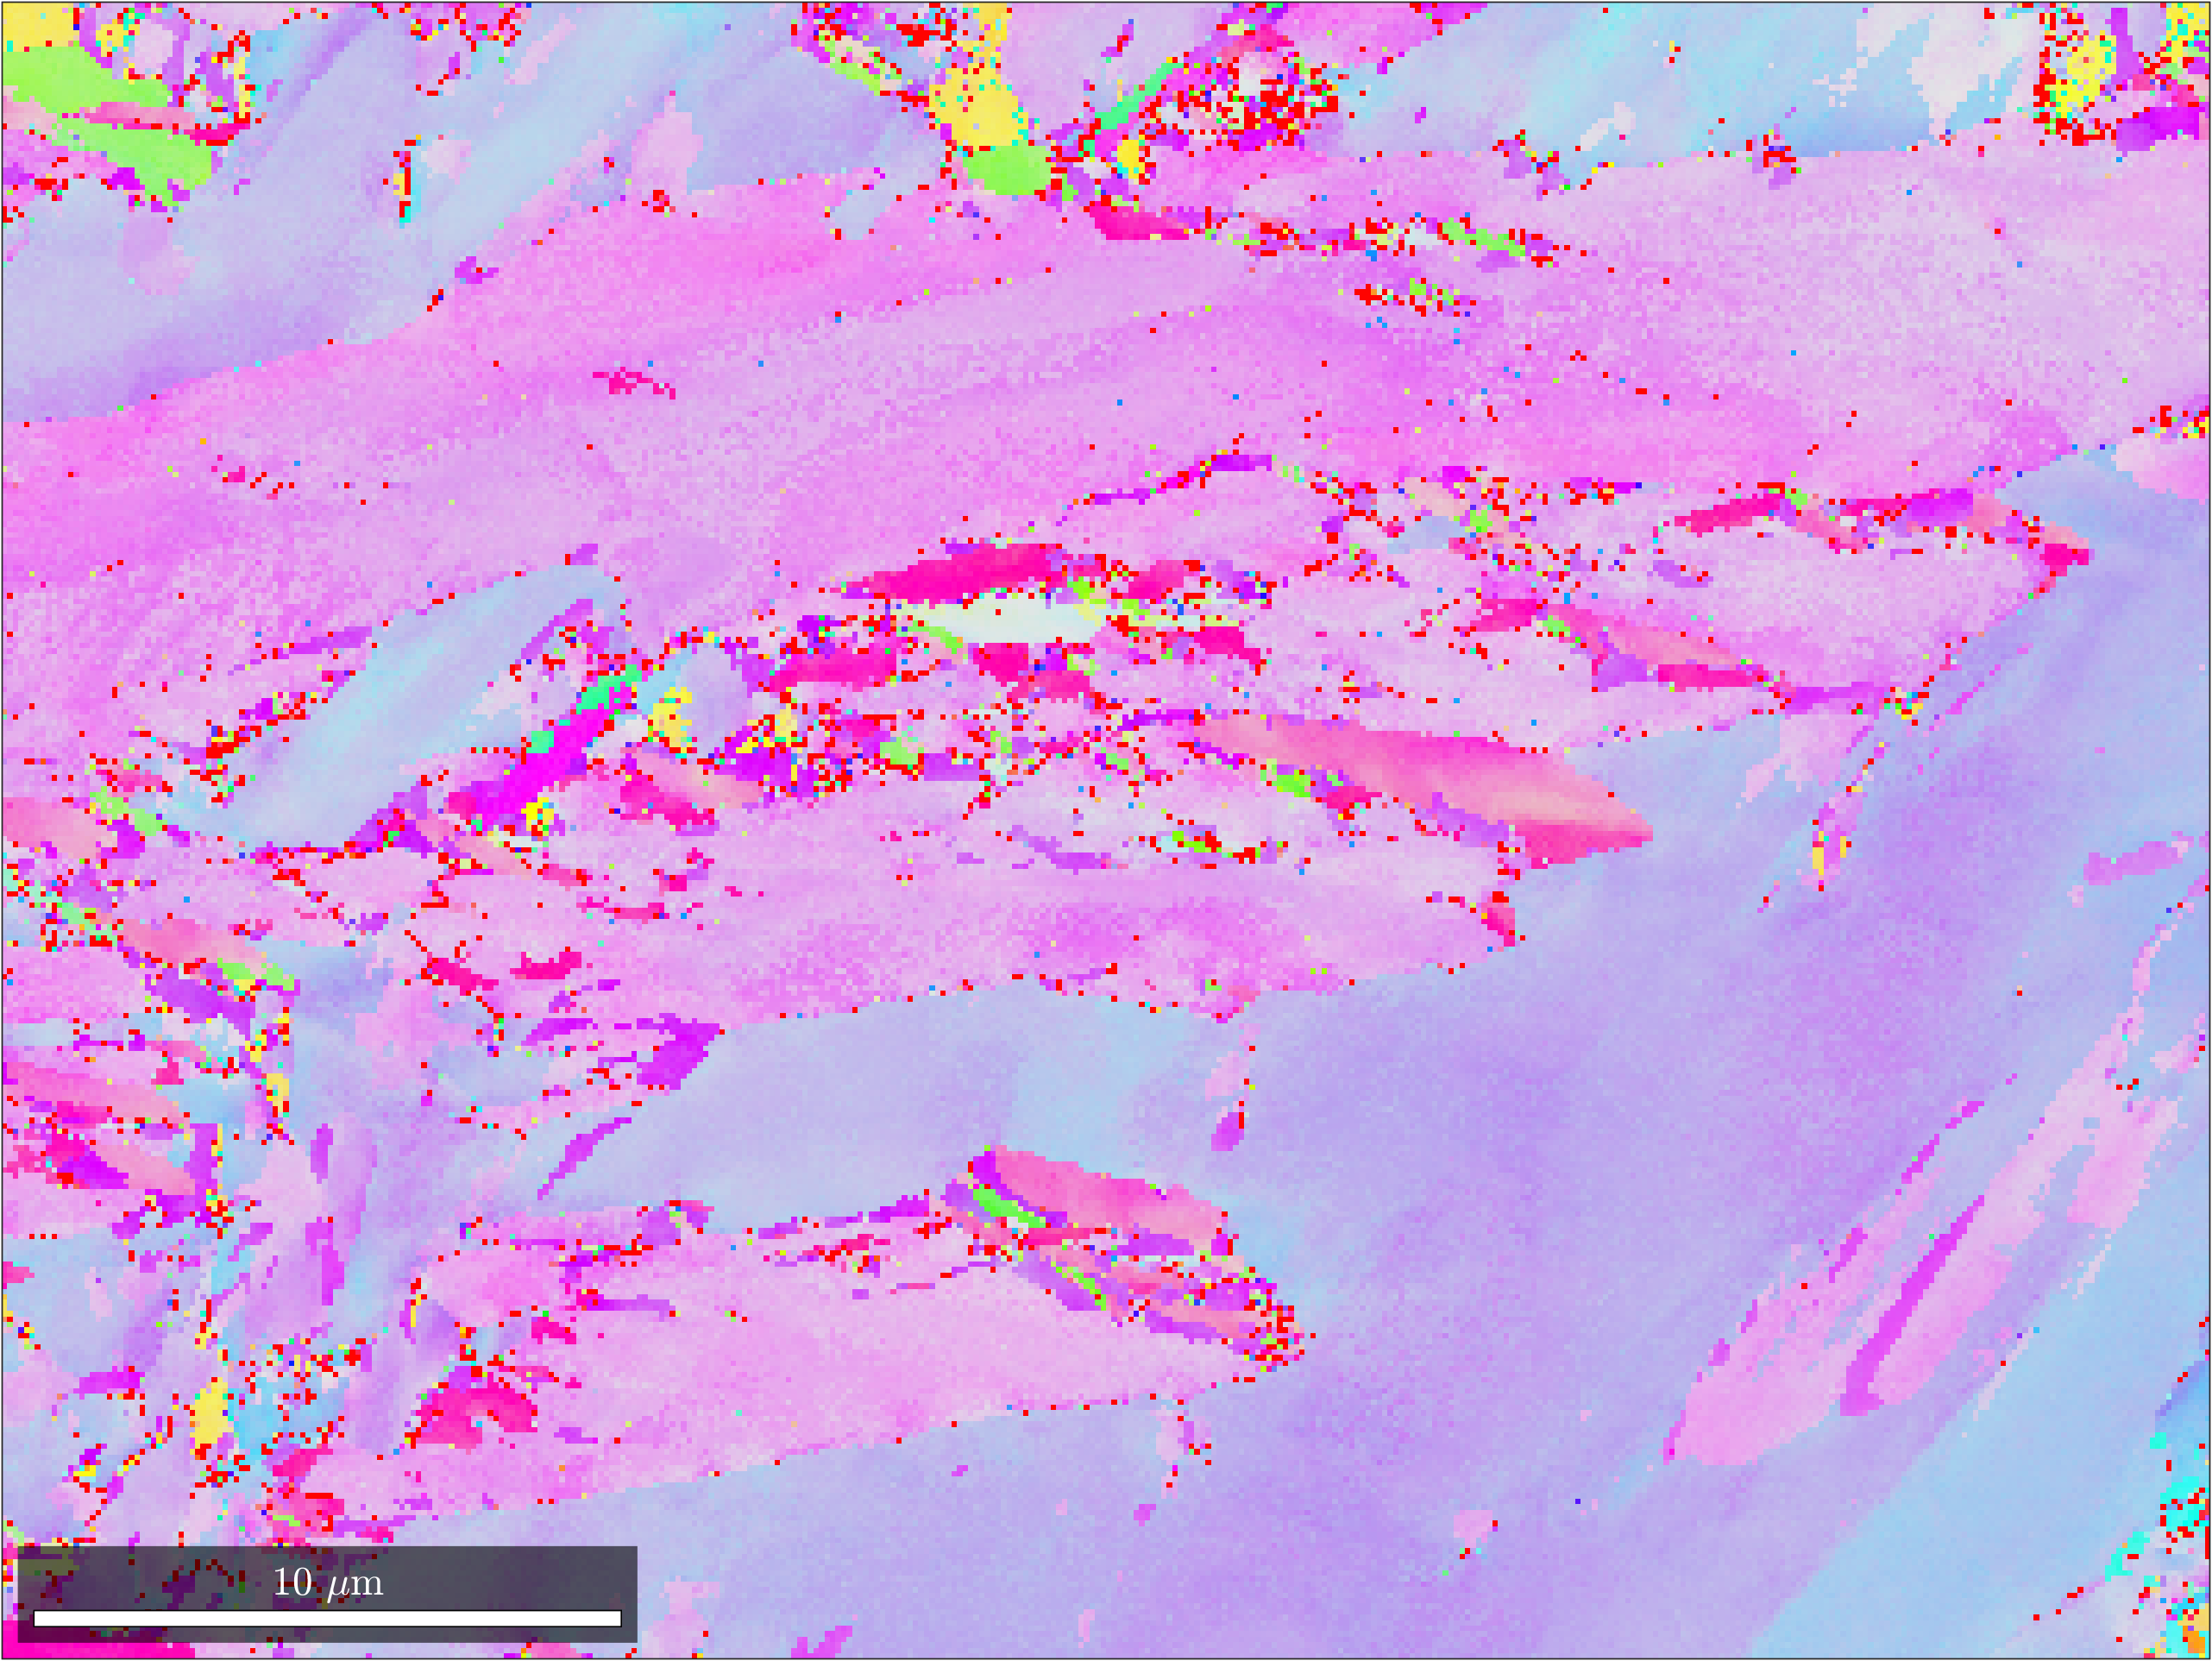
\includegraphics[width=0.49\textwidth]{pic2/nolze/raw}
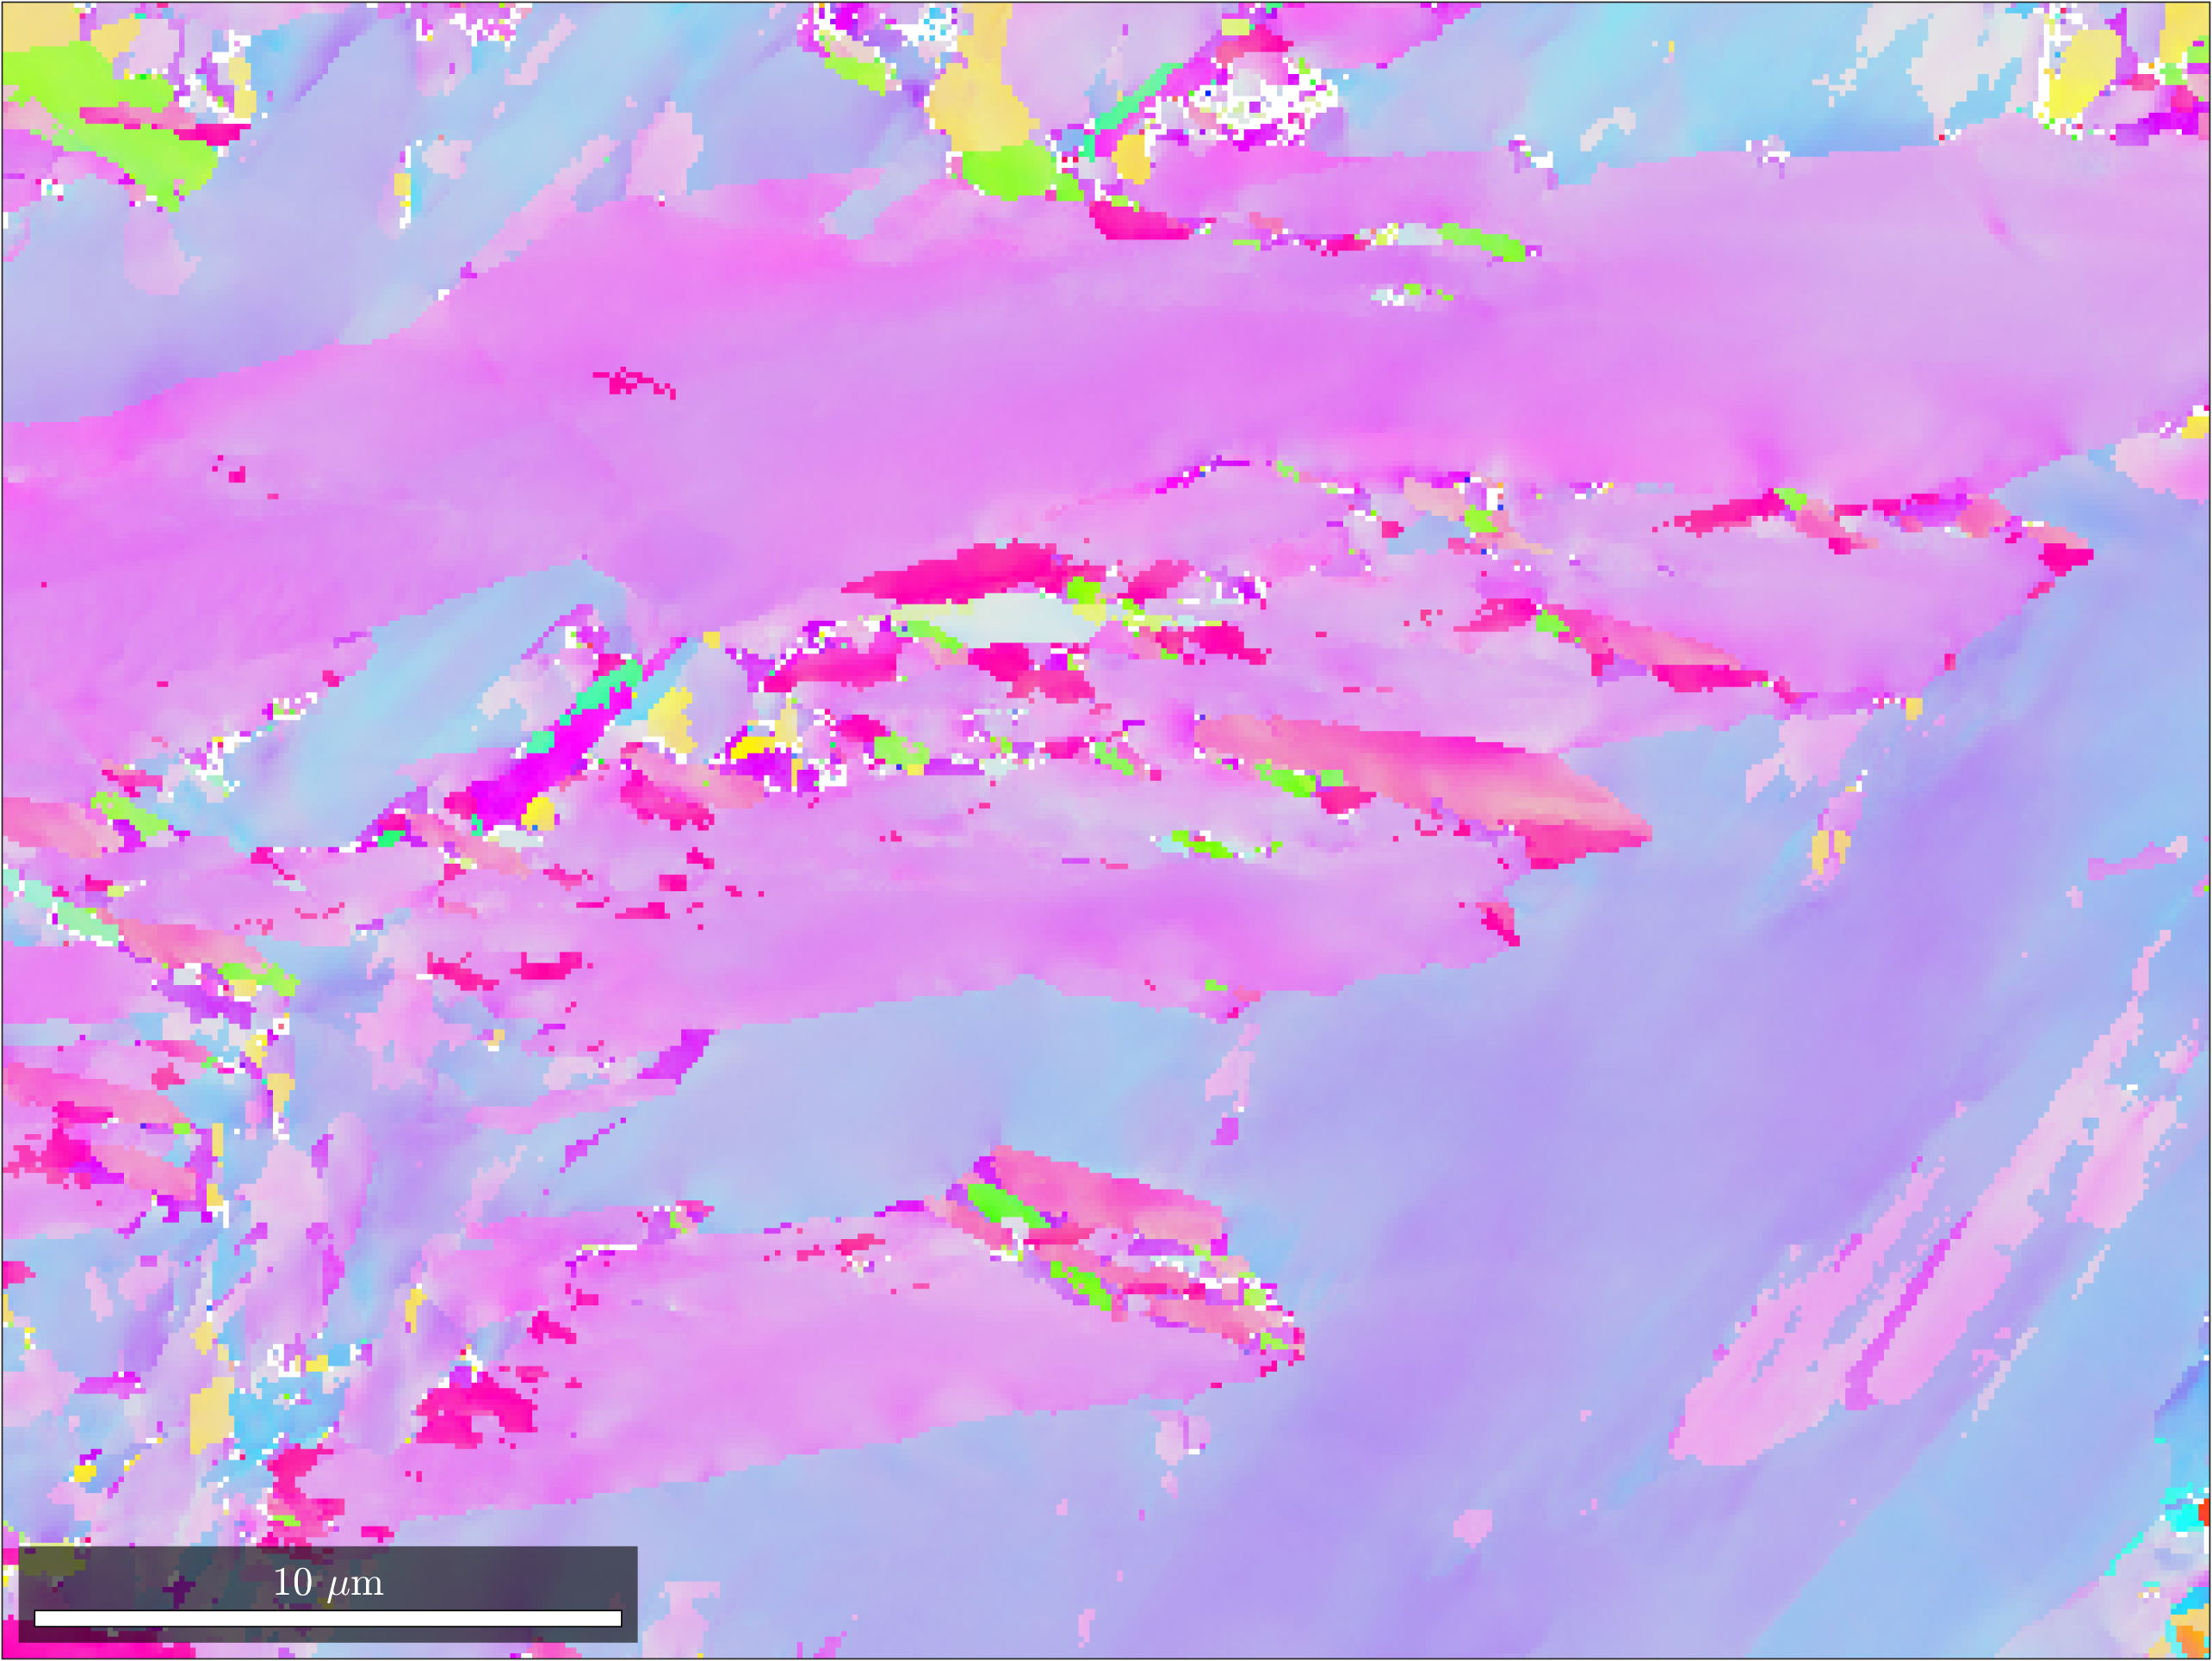
\includegraphics[width=0.49\textwidth]{pic2/nolze/refined}

\end{frame}

\begin{frame}

  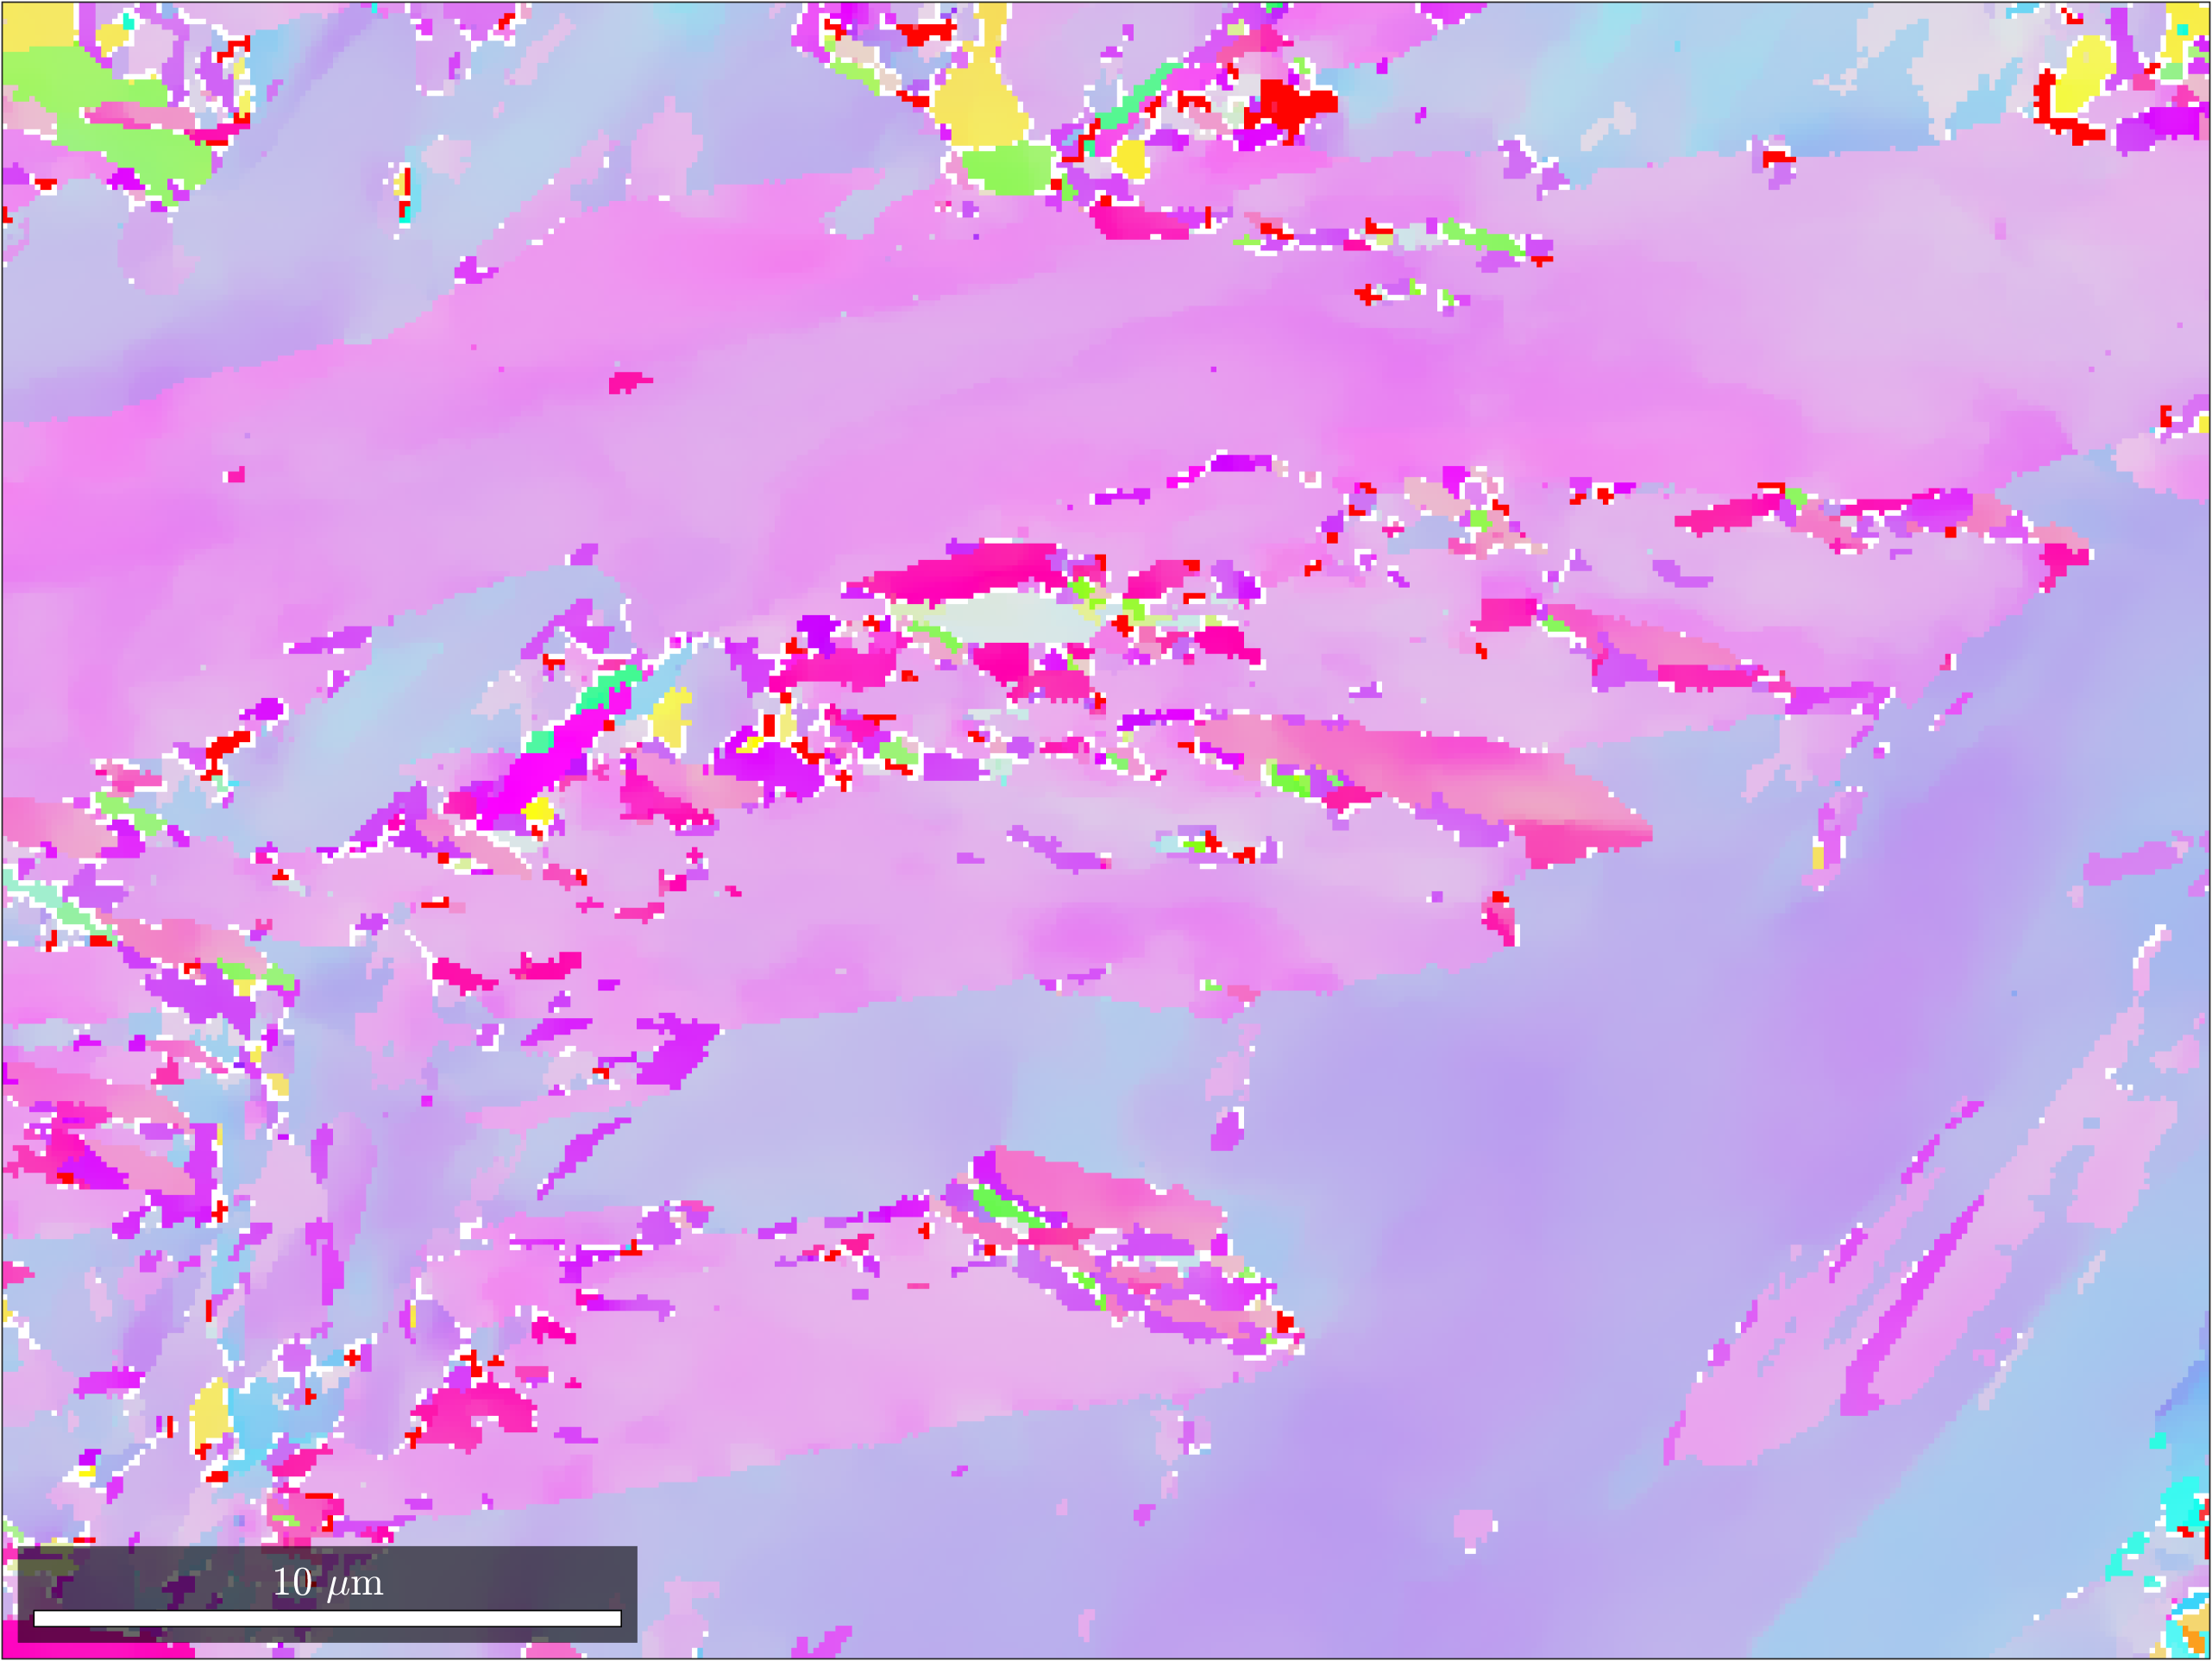
\includegraphics[width=0.49\textwidth]{pic2/nolze/denoised}
  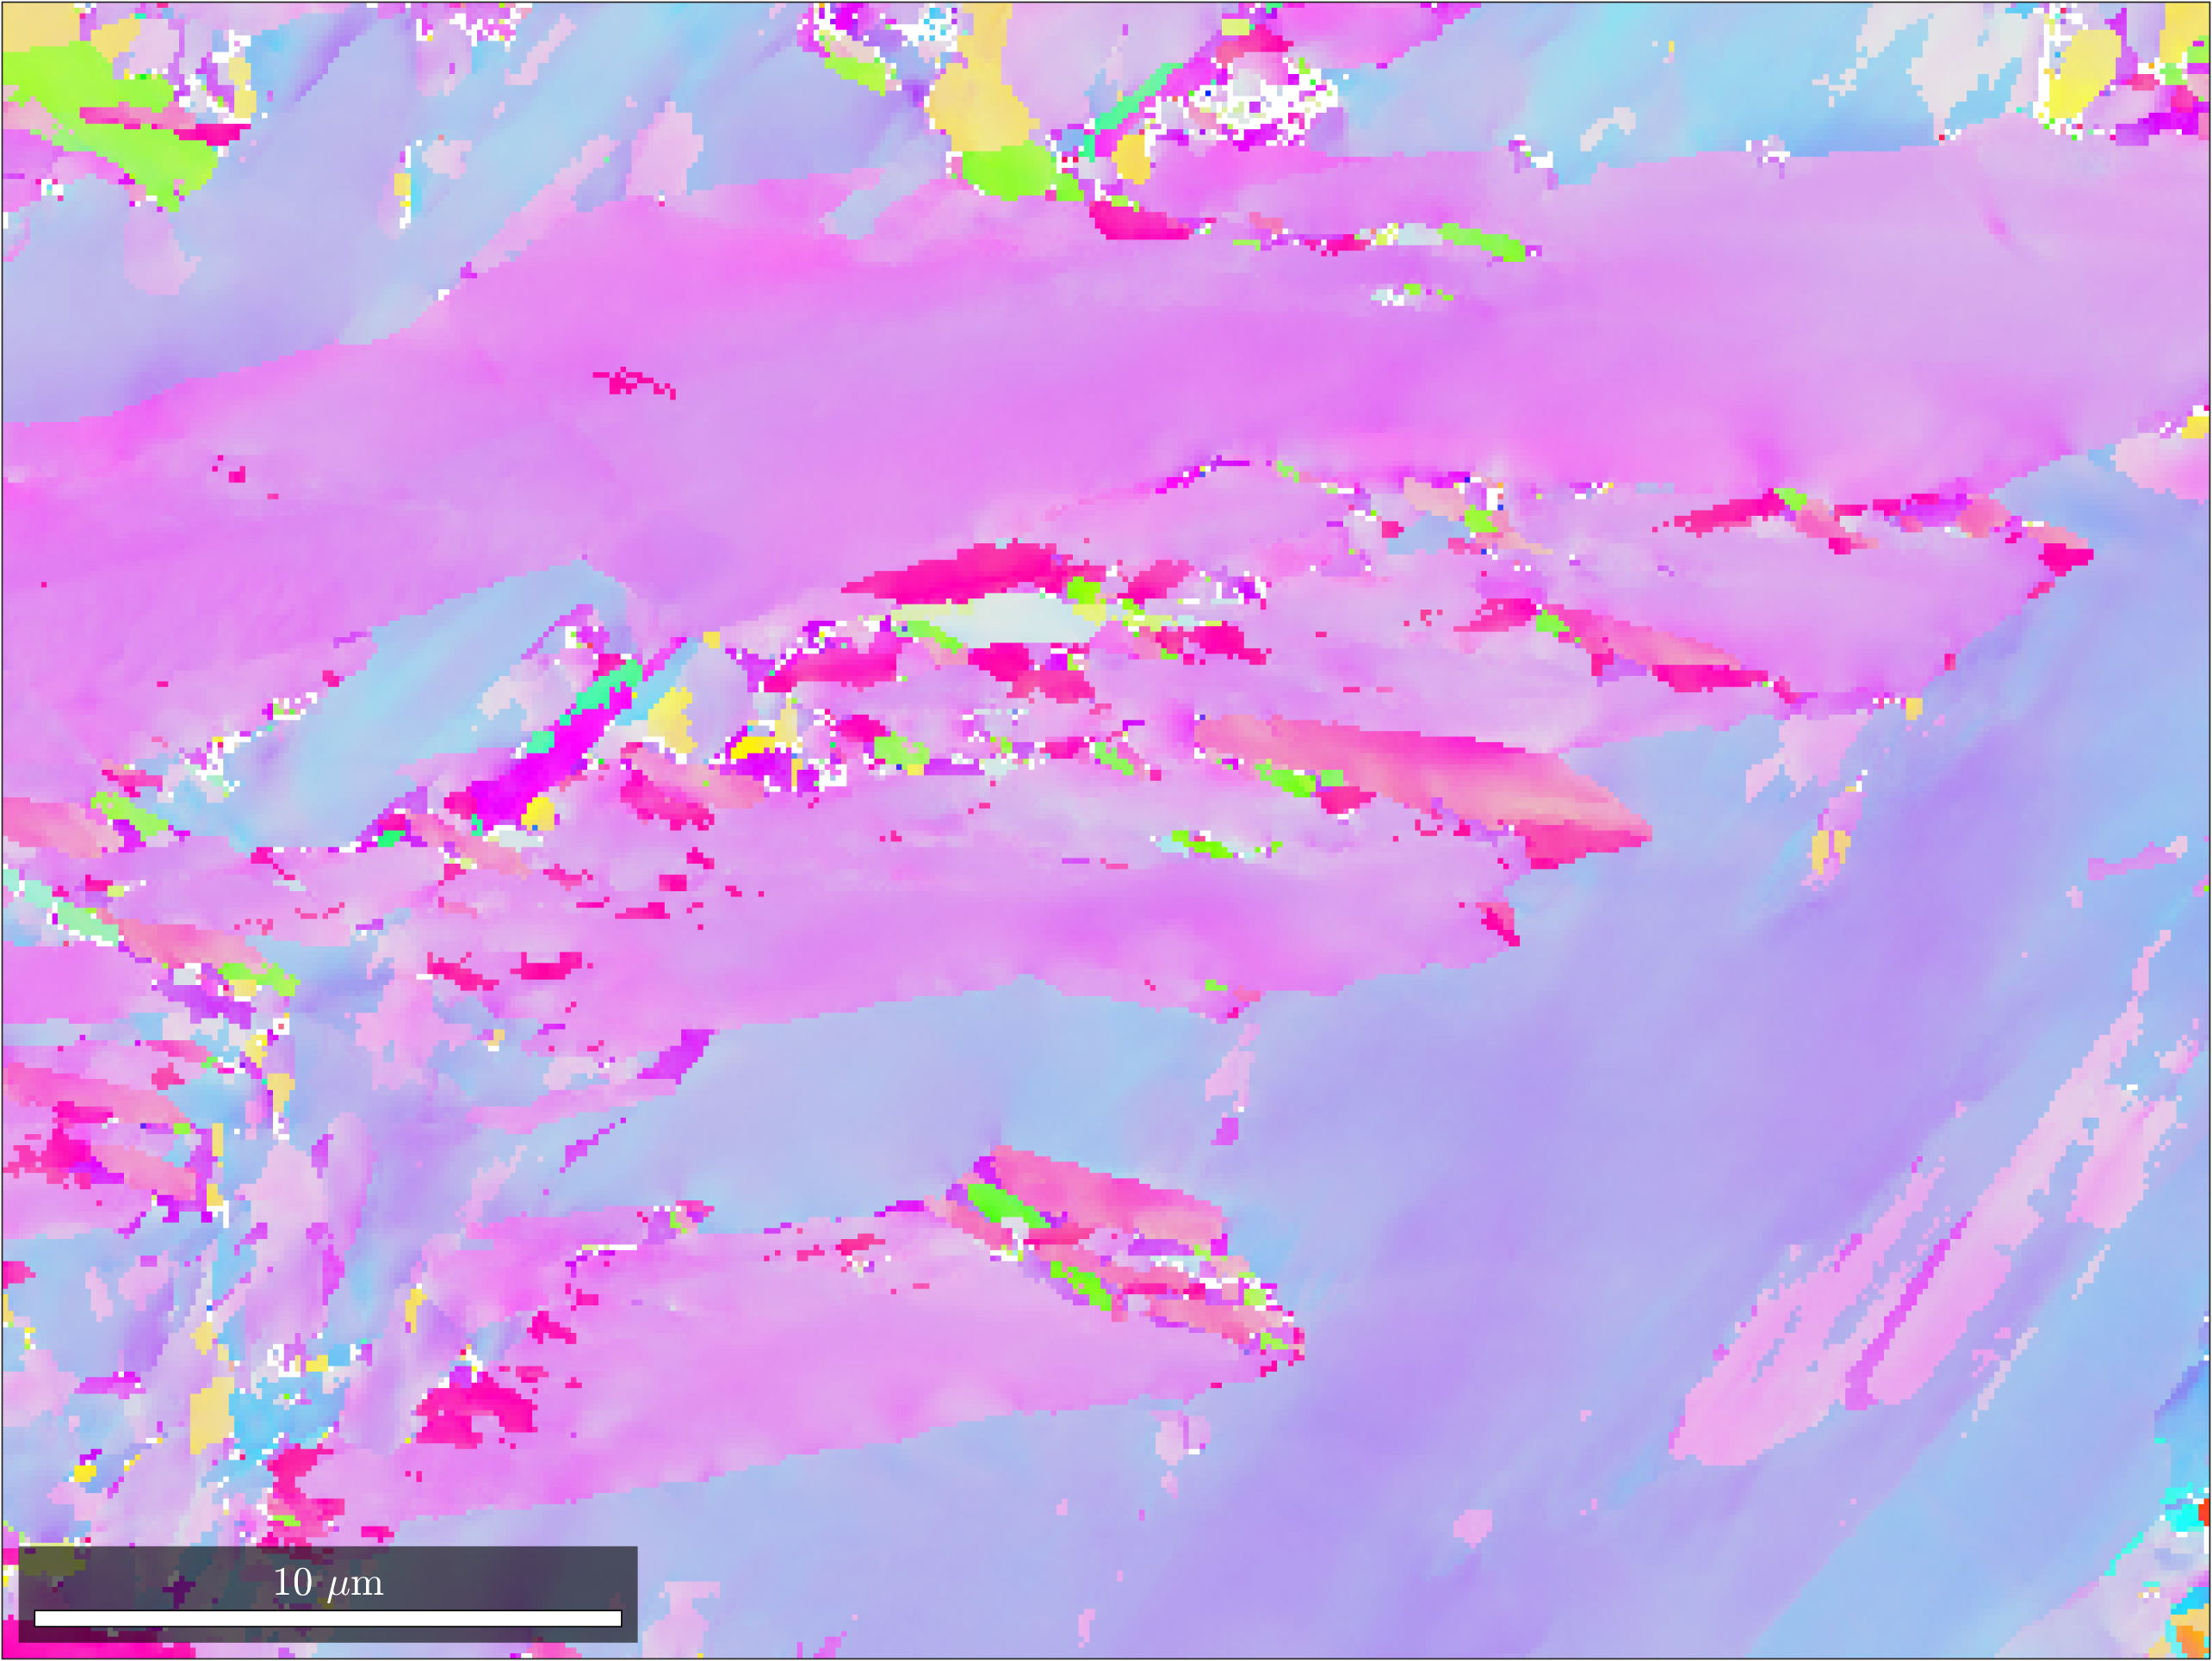
\includegraphics[width=0.49\textwidth]{pic2/nolze/refined}

\end{frame}

\begin{frame}
  \frametitle{Comparison of Curvature Maps}

  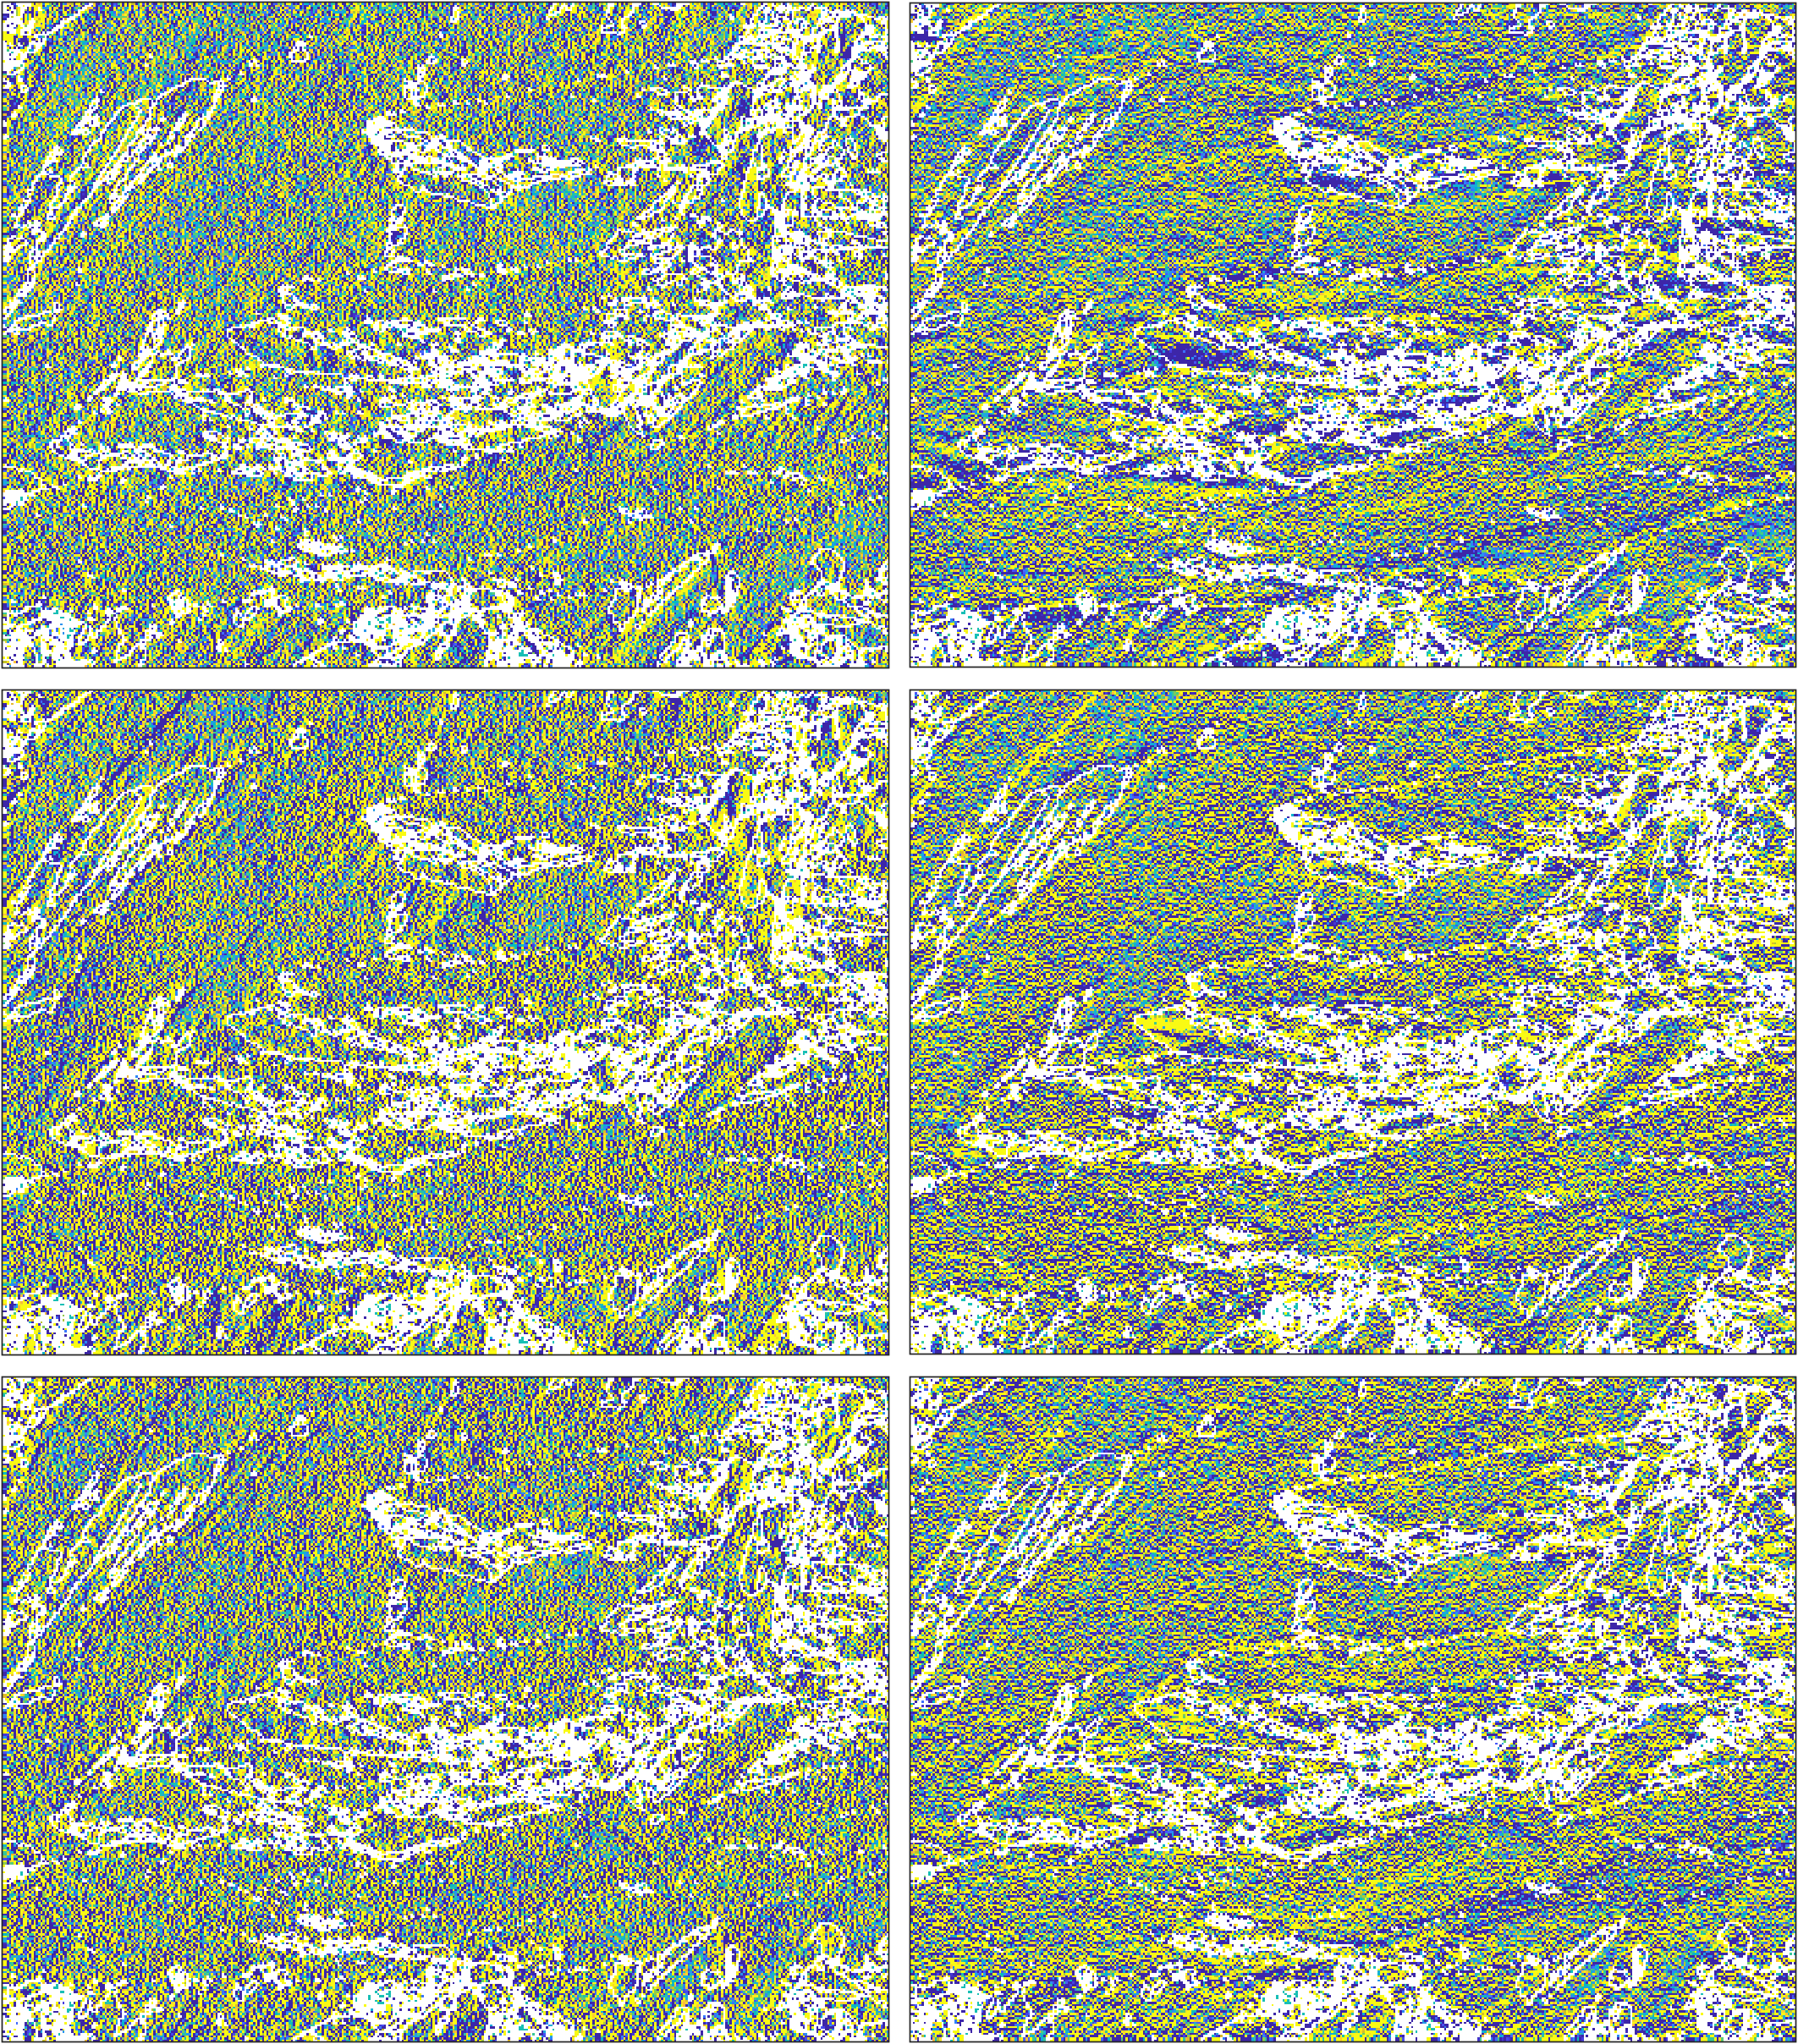
\includegraphics[width=0.32\textwidth]{pic2/nolze/kappaRaw}
  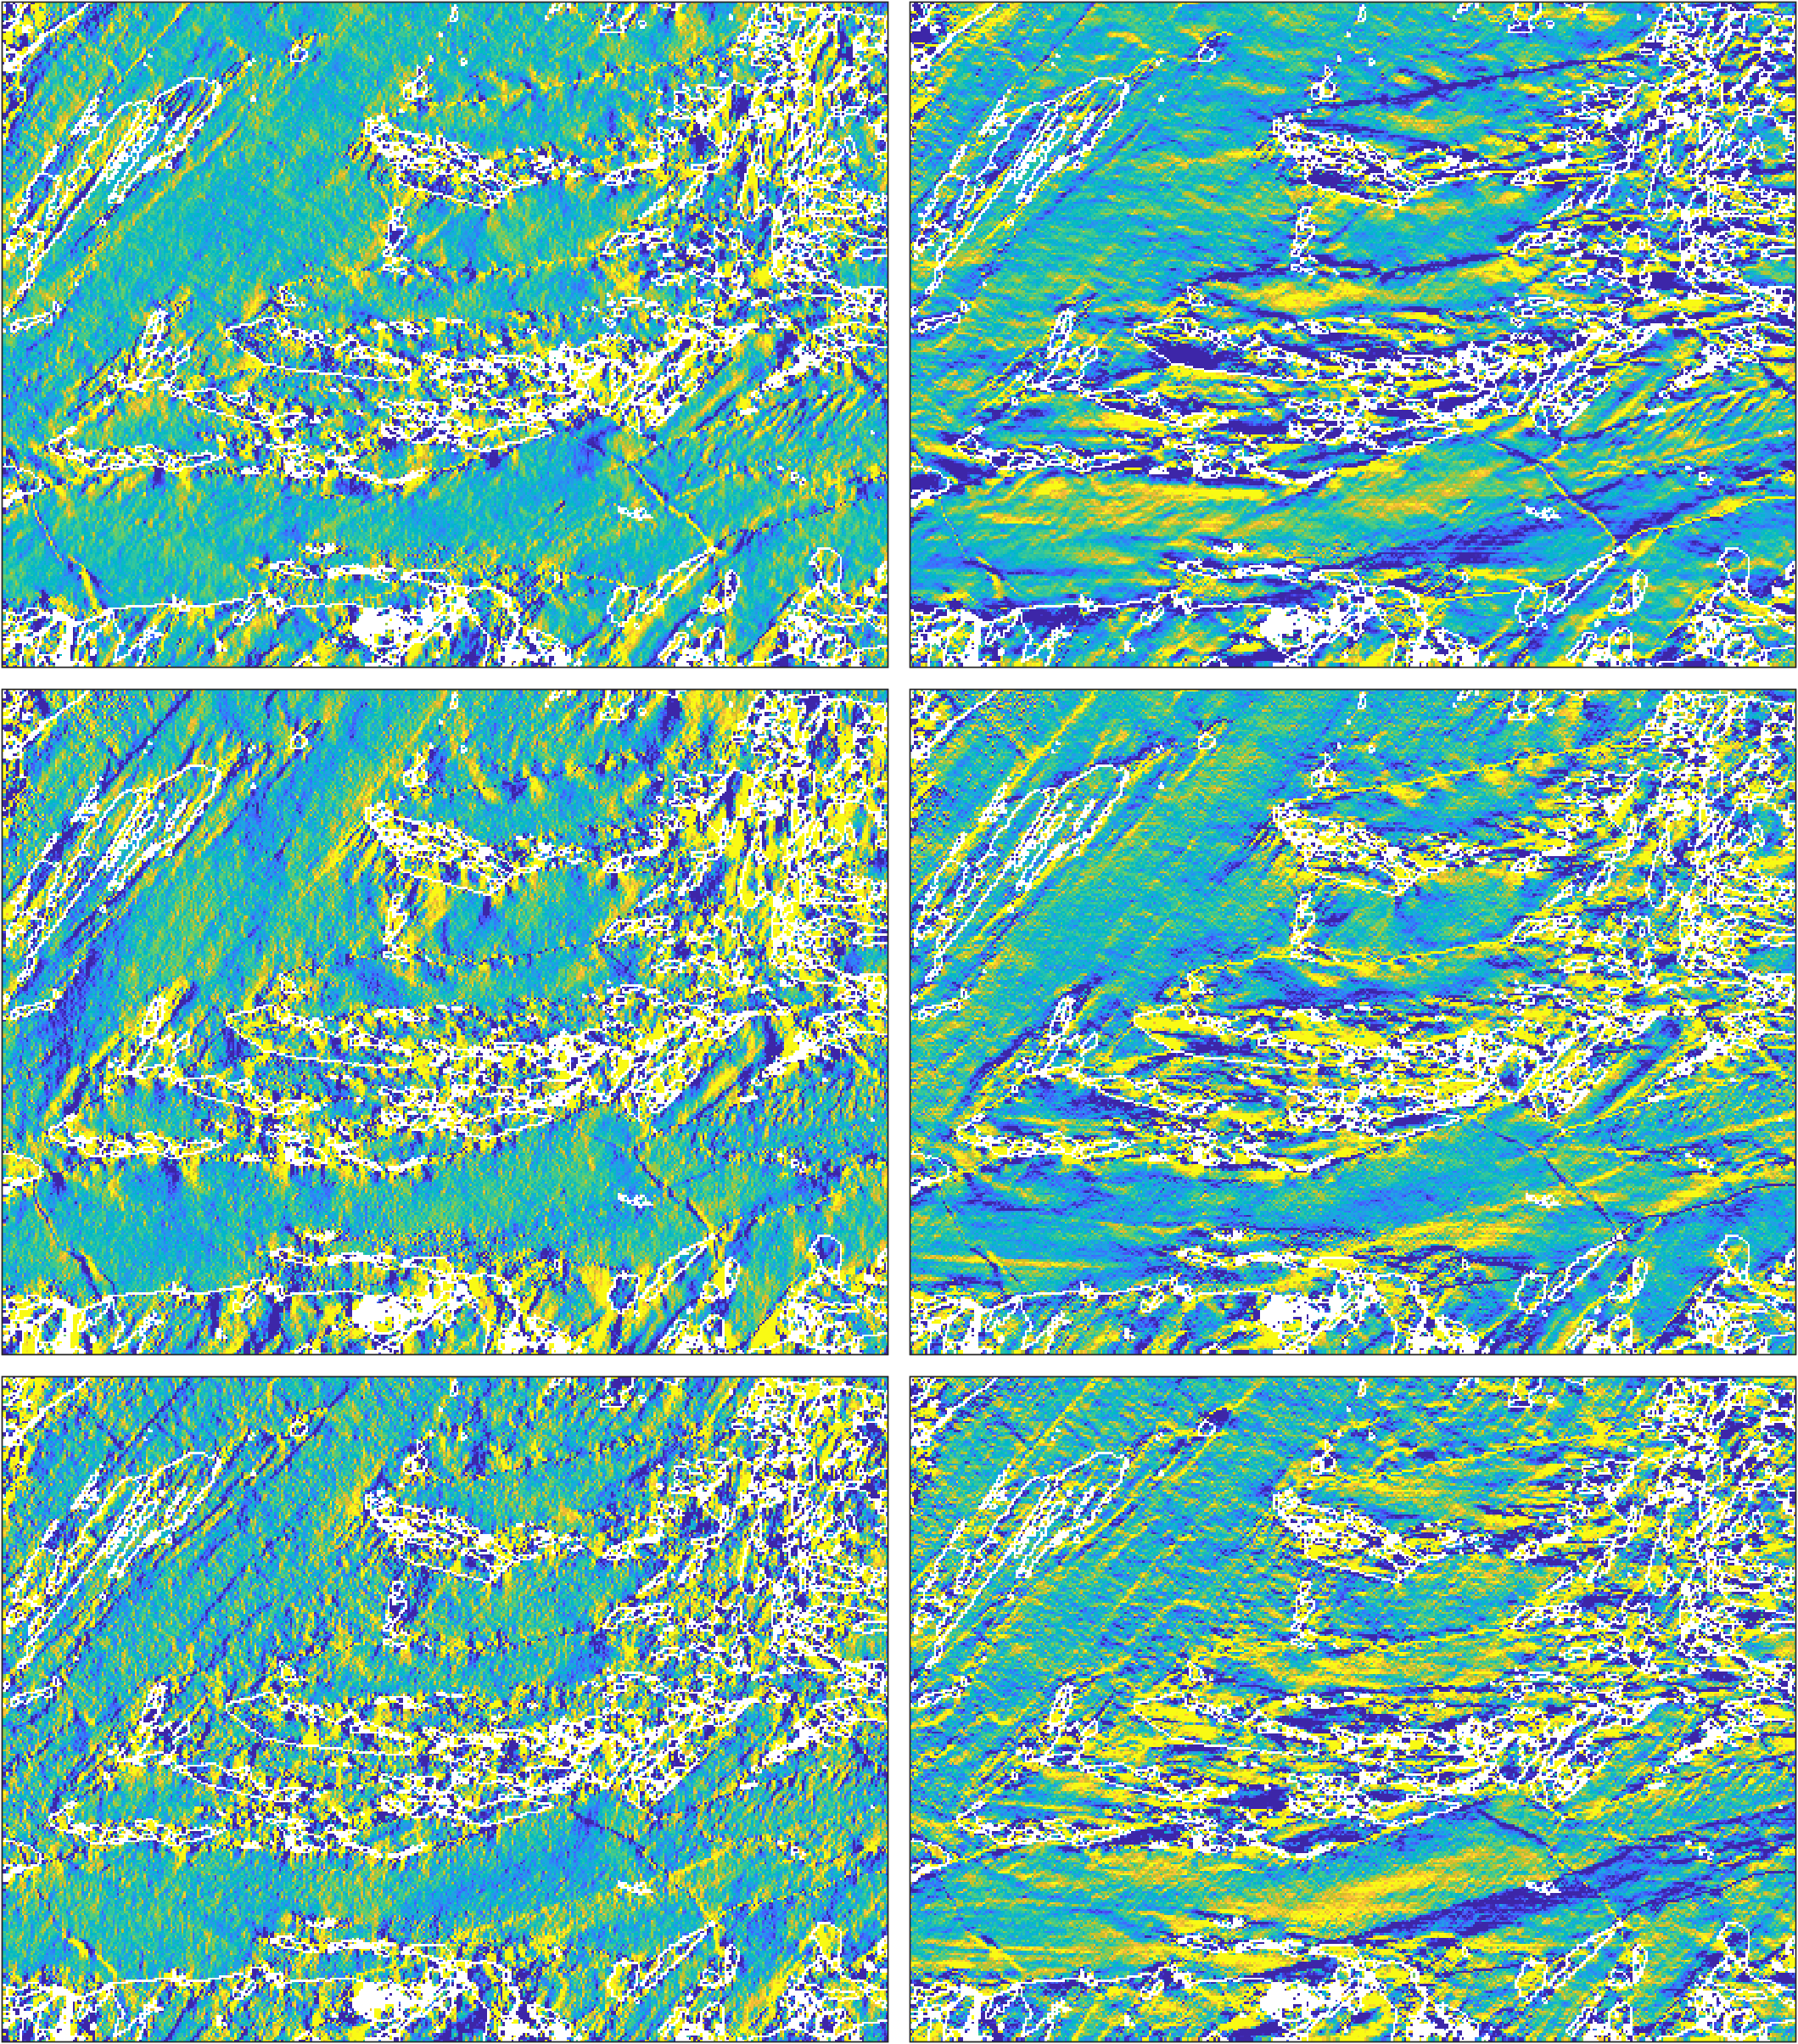
\includegraphics[width=0.32\textwidth]{pic2/nolze/kappaRefined}
  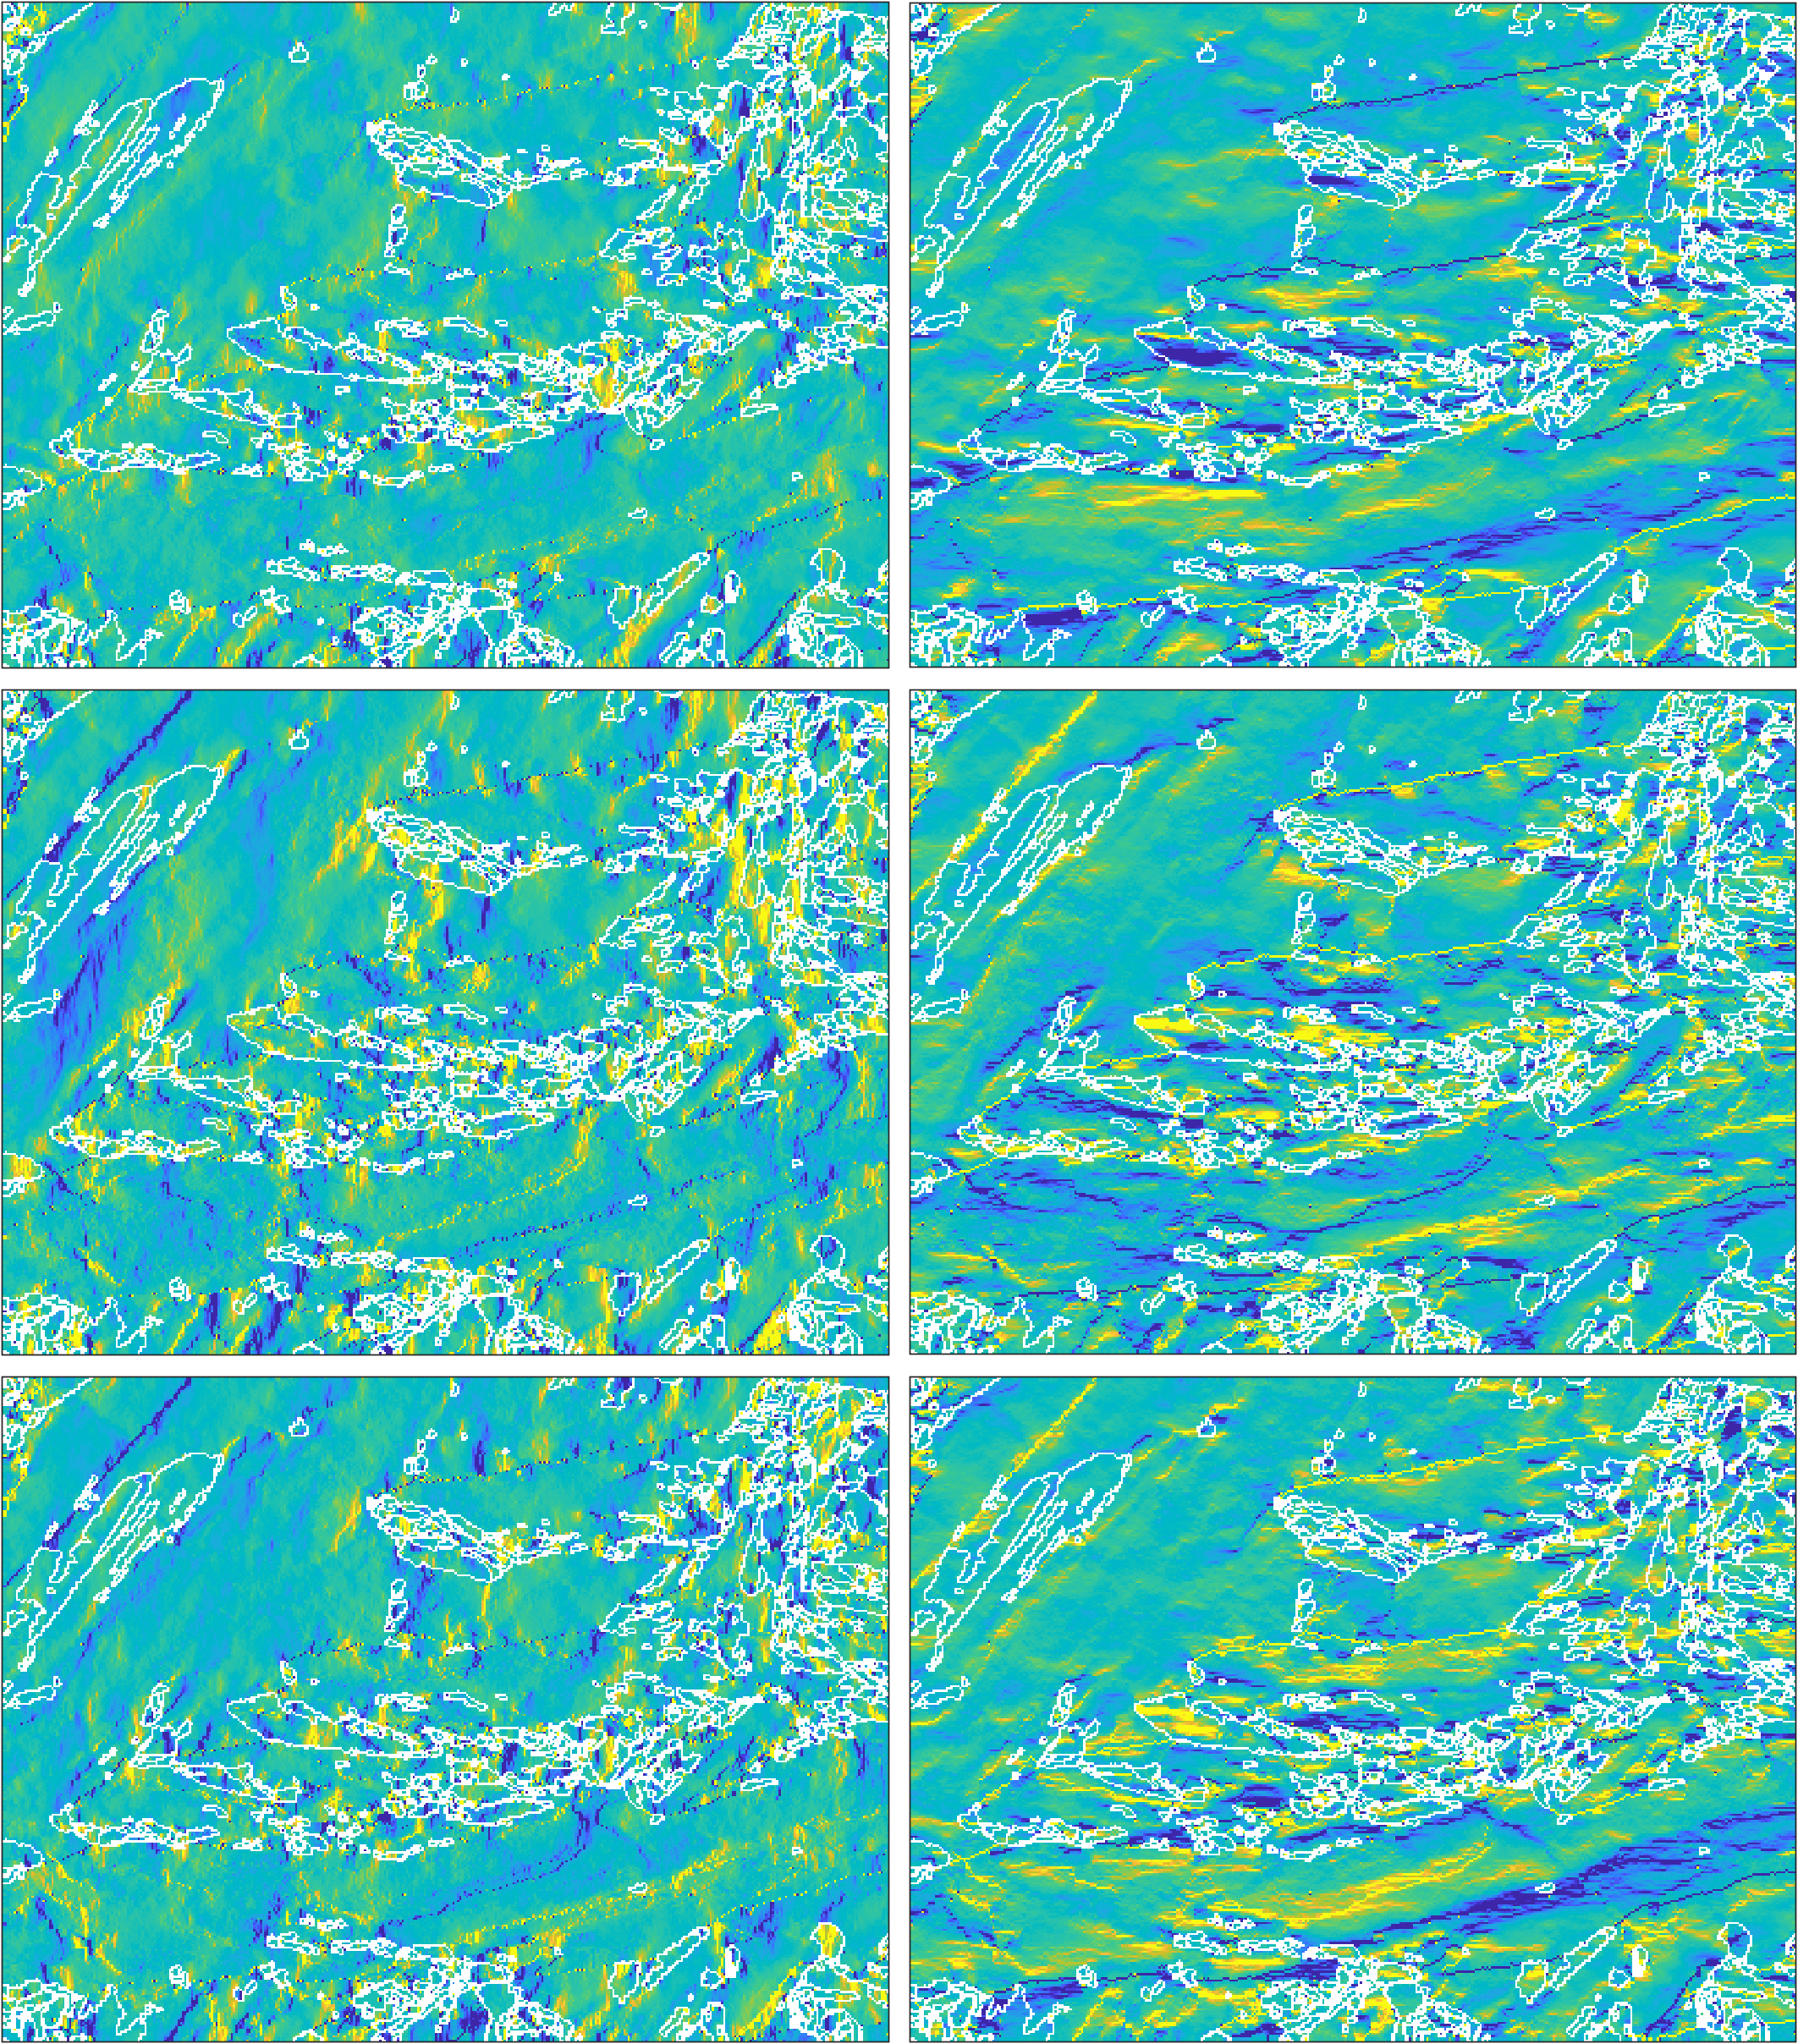
\includegraphics[width=0.32\textwidth]{pic2/nolze/kappaDenoised}

\end{frame}



\end{document}


%%% Local Variables:
%%% mode: latex
%%% TeX-master: t
%%% End:

\begin{frame}[fragile]
  \frametitle{Some Smoothing Techniques}

  \vspace{-0.6cm}
  \begin{overlayarea}{\textwidth}{\textheight}
  \begin{columns}
    \begin{column}{8.3cm}
        \begin{enumerate}
        \item<+-> \structure{Mean Filter:} mean orientation
          of neighbors
        \item<+-> \structure{Median Filter:}  neighboring
          orientation with minimum distance to all other neighboring
          orientations
        \item<+-> \structure{Smoothing Splines:} % Given orientation map $O_{ij}$,
          % determine smoothed map $\tilde O_{ij}$ as solution of the
          % minimization problem
          \begin{equation*}
            \sum_{i,j} \omega(O_{ij},\tilde O_{ij})^{2} + \alpha \nabla
            \tilde O_{ij}^{2} \to \min
          \end{equation*}
        \item<+-> \structure{Half Quadratic Optimization:}
          \begin{equation*}
            \sum_{i,j} \omega(O_{ij},\tilde O_{ij})^{2} + \alpha \left|\nabla
            \tilde O_{ij}\right| \to \min
        \end{equation*}
      \item<+-> \structure{Infimal Convolution:}
          \begin{equation*}
            \sum_{i,j} \omega(O_{ij},\tilde U_{ij} \tilde V_{ij})^{2} + \alpha \left|\nabla
            \tilde U_{ij}\right| + \beta  \left|\triangle
            \tilde V_{ij}\right| \to \min
          \end{equation*}
        \end{enumerate}
    \end{column}
    \begin{column}{3.8cm}
      \begin{onlyenv}<1>
        
\includegraphics[width=\textwidth]{pic2/ebsd1mis2meanMean.png}\\
        \includegraphics[width=\textwidth]{pic2/oMSharp1.png}
      \end{onlyenv}
      \begin{onlyenv}<2>
        
\includegraphics[width=\textwidth]{pic2/ebsd1mis2meanMedian.png}\\
        \includegraphics[width=\textwidth]{pic2/oMSharp1.png}
      \end{onlyenv}
      \begin{onlyenv}<3>
        
\includegraphics[width=\textwidth]{pic2/ebsd1mis2meanSmooth.png}\\
        \includegraphics[width=\textwidth]{pic2/oMSharp1.png}
      \end{onlyenv}
      \begin{onlyenv}<4>
        
\includegraphics[width=\textwidth]{pic2/ebsd1mis2meanHalfQuad.png}\\
        \includegraphics[width=\textwidth]{pic2/oMSharp1.png}
      \end{onlyenv}
      \begin{onlyenv}<5>
        
\includegraphics[width=\textwidth]{pic2/ebsd1mis2meanInfimal.png}\\
        \includegraphics[width=\textwidth]{pic2/oMSharp1.png}
      \end{onlyenv}
    \end{column}
  \end{columns}
    \end{overlayarea}
\end{frame}

\end{document}

\begin{frame}[fragile]
  \frametitle{Phase Transition}

  The Burger OR translates beta into alpha coordinates
  \vspace{-0.2cm}
  \begin{lstlisting}[style=input]
b2a = orientation.burger(csBeta,csAlpha)
b2a * Miller(0,0,1,csBeta)
  \end{lstlisting}
  \begin{lstlisting}[style=output]

  \end{lstlisting}

\medskip
\pause

consider an alpha orientation
  \vspace{-0.2cm}
\begin{lstlisting}[style=input]
oriAlpha = orientation.Id(csAlpha)
oriAlpha * b2a * Miller(0,0,1,csBeta)
\end{lstlisting}

\medskip
\pause

Hence, we can compute a beta orientation out of
  \vspace{-0.2cm}
\begin{lstlisting}[style=input]
oriBeta = oriAlpha * b2a
\end{lstlisting}

\medskip
\pause

conversely, we obtain an alpha orientation by
  \vspace{-0.2cm}
\begin{lstlisting}[style=input]
oriAlpha = oriBeta * inv(b2a)
\end{lstlisting}


\end{frame}


\begin{frame}[fragile]
  \frametitle{Variants}

  \begin{columns}
    \begin{column}{0.7\textwidth}
      \begin{overlayarea}{\textwidth}{0.85\textheight}

      Due to symmetry the Burger OR translates a single beta orientation into
      several alpha orientations \vspace{-0.2cm}
  \begin{lstlisting}[style=input]
oriAlpha = oriBeta * inv(b2a.symmetrise)
oriAlpha = oriBeta.symmetrise * inv(b2a)
\end{lstlisting}

\medskip
\pause

Some of these alpha orientations at not symmetrically equivalent.
The are called variants of \texttt{oriBeta}
  \vspace{-0.2cm}
\begin{lstlisting}[style=input]
alphaV = variants(b2a, oriBeta)
\end{lstlisting}

\medskip
\pause

Lets compare alpha and beta orientations
    \vspace{-0.2cm}
\begin{lstlisting}[style=input]
plotPDF(oriBeta,Miller(1,1,0,csBeta))
hAlpha = symmetrise(Miller(0,0,0,1,csAlpha)
plotPDF(alphaV * hAlpha)
\end{lstlisting}

\begin{onlyenv}<15>
determine which variant we have
    \vspace{-0.2cm}
\begin{lstlisting}
id = calcVariantId(oriBeta,oriAlpha,b2a)
\end{lstlisting}
\end{onlyenv}



      \end{overlayarea}

\end{column}
\begin{column}{0.23\textwidth}
  \begin{overlayarea}{\textwidth}{0.85\textheight}
    \vspace{-0.75cm}
\centering
\only<3>{
\includegraphics[width=\textwidth]{pic2/varPf1}}
\only<4>{
\includegraphics[width=\textwidth]{pic2/varPf2}}
\only<5>{
\includegraphics[width=\textwidth]{pic2/varPf3}}
\only<6>{
\includegraphics[width=\textwidth]{pic2/varPf4}}
\only<7>{
\includegraphics[width=\textwidth]{pic2/varPf5}}
\only<8>{
\includegraphics[width=\textwidth]{pic2/varPf6}}
\only<9>{
\includegraphics[width=\textwidth]{pic2/varPf7}}
\only<10>{
\includegraphics[width=\textwidth]{pic2/varPf8}}
\only<11>{
\includegraphics[width=\textwidth]{pic2/varPf9}}
\only<12>{
\includegraphics[width=\textwidth]{pic2/varPf10}}
\only<13>{
\includegraphics[width=\textwidth]{pic2/varPf11}}
\only<14>{
\includegraphics[width=\textwidth]{pic2/varPf12}}
\only<15>{
\includegraphics[width=\textwidth]{pic2/varPf}}
\end{overlayarea}
\end{column}
  \end{columns}


\end{frame}


\begin{frame}[fragile]
  \frametitle{Child to Child Misorientations}

    \begin{columns}
    \begin{column}{0.7\textwidth}
      \begin{overlayarea}{\textwidth}{0.85\textheight}
        assume two child variants
        \begin{itemize}
        \item \texttt{oriA1 = oriB * SymB1 *  inv(b2a)}
        \item \texttt{oriA2 = oriB * SymB2 *  inv(b2a)}
        \end{itemize}
        \pause
        \medskip
        then its misorientation is
        \vspace{-0.2cm}
        \begin{align*}
        &\mathtt{inv(oriA1)*oriA2}\\
        &= \mathtt{b2a * symB1 * inv(oriB) * oriB * symB2 * inv(b2a)} \\
        &= \mathtt{b2a * symB * inv(b2a)}
        \end{align*}

        \pause

        list of all possibe child to child misorientations
        \vspace{-0.2cm}
        \begin{lstlisting}[style=input]
c2c = b2a.variants * b2a
        \end{lstlisting}

        \pause
        compute fit and parent orientation
        \vspace{-0.2cm}
        \begin{onlyenv}<5>
        \begin{lstlisting}[style=input]
[oriB, fit] = calcParent([oriA1,oriA2], b2a)
\end{lstlisting}
        \end{onlyenv}

        \begin{onlyenv}<6>
\begin{lstlisting}[style=input]
oriA = orientation.rand(1000,2,csAlpha);
[~,fit] = calcParent(oriA,beta2alpha);
\end{lstlisting}
\end{onlyenv}

        \begin{onlyenv}<7>
\begin{lstlisting}[style=input]
oriA = orientation.rand(1000,3,csAlpha);
[~,fit] = calcParent(oriA,beta2alpha);
\end{lstlisting}
\end{onlyenv}
\end{overlayarea}
    \end{column}
    \begin{column}{0.3\textwidth}
      \begin{overlayarea}{\textwidth}{0.85\textheight}

        \vspace{-0.75cm}
        \begin{onlyenv}<6>
          
\includegraphics[width=\textwidth]{pic2/fitHist}


          
\includegraphics[width=\textwidth]{pic2/fit2}
        \end{onlyenv}

        \begin{onlyenv}<7>

          
\includegraphics[width=\textwidth]{pic2/fitHist3}


          
\includegraphics[width=\textwidth]{pic2/fit3}
      \end{onlyenv}
    \end{overlayarea}
    \end{column}
  \end{columns}
\end{frame}


% \begin{frame}[fragile]
%   \frametitle{Merging Grains}

%   \begin{lstlisting}
% % merge according to grain boundary misorientations
% gB = grains.boundary('Mag','Hem')
% isParent2Child = angle(gB.meanOrientation, Mag2Hem) < 2*degree;
% [grains_merged, parentId] = merge(grains,gB(isParent2Child))

% % merge according to triple points
% tP = grains.triplePoints('Hem','Hem','Hem')
% isChildTP = ... % some condition
% [grains_merged, parentId] = merge(grains,tP(isChildtp))

% % merge according to a pairs list
% pairs = [1 2 ; ...
%          1 3 ; ...
%          4 8 ; ...
%          5 6]
% [grains_merged, parentId] = merge(grains,pairs)
%   \end{lstlisting}
% \end{frame}



\end{document}
